\chapter{Data}
\label{chap:three}
% grammar checked (07-27)

\section{Literature search}
\label{sec:literature_search}

I make use of the Google Scholar search engine with its full-text search capabilities to assemble my dataset. A query constructed using a combination of keywords helps me narrow down the results into studies dealing with ability bias, private returns, and education. After several modifications to ensure the query generates consistent results within the scope of interest, I finalized the query into a form denoted in \autoref{app:one}.

I ran the definitive search on January 23, 2023, and received 574 hits. To achieve absolute consistency, I employed web scraping and automatic data pre-processing tools and denoted all vital information about all 574 studies during a single day. These included the authors' names, publication information, the number of citations, and the impact factor of the journal the study was published in\footnote{In case of an unpublished study, I set the impact factor to 0.}. To avoid duplicate results and guarantee the uniqueness of each hit, I also extracted the study result IDs.

I then went through the first 200 studies and deemed 78 as eligible for data collection. For this preliminary check, I considered only whether each study was relevant to the topic, and whether it reported the necessary statistics, namely an estimate of a returns to schooling regression, the corresponding standard error, etc.
Although a sizable number of studies failed to report collectible data completely, 129 of the 200 studies (over 60\% of the surveyed sample) were at least relevant to the topic, validating thus the quality of my query.

In accordance with the reporting guidelines for meta-analysis by \cite{havranek2020guidelines}, I define the following criteria that will help me narrow down the study list into its final form. For a study to be included in the dataset, it must fulfill the following criteria.

First, the study must report one or more estimates from an equation of any form of wage on a schooling variable (years of schooling or completed level of education), along with their standard errors or corresponding t-statistics. Without the last two mentioned, there would be no way to compare effect strength across observations. Furthermore, there must either be a traceable statistic associated with every estimate that signifies the number of degrees of freedom or sample size from the regression or, in case neither of these is provided, there must be a number denoting the number of subjects for the experiment. In such cases, it must be evident that the sample size corresponds to the reported estimates. Due to the thoroughness of the initial screening, only four studies of the 78 did not fulfill these criteria and were thus removed. This leaves a total of 74 studies eligible for collection.

To retain as much information about the research field as possible, I choose \textit{not} to discard studies of varying quality, including unpublished papers, graduate theses, dissertations, etc. There is no consensus in the existing literature on which approach should be taken, as highlighted by \cite{stanley2001wheat}. Even though the author advises careful consideration when including unpublished studies, he also acknowledges that their omission could create a new publication bias instead. The inclusion approach is also supported by \cite{cook1993should}, who found that numerous meta-analysis researchers and methodologists believe data from unpublished studies should not be discarded if one aims to synthesize the available information objectively.

However, upon closer inspection of the initially generated list of studies, I observed that several highly influential studies from the field were missing, such as those by  \cite{angrist1991compulsory}, \cite{staiger1997instrumental}, or \cite{heckman2006earnings}. These failed to get identified as relevant by the query and did not appear in the search results. To ensure the whole field of relevant literature is encompassed, I employ the snowballing method to incorporate these crucial studies.

The use of the snowballing method itself is debatable too , and an argument can be made for its avoidance, as the data search suddenly becomes hard to replicate. Indeed, having only one search query would be ideal, but the unfortunate failure of the query to detect many of the most important studies in the field seemed a reason enough to give snowballing a green flag. As an example, the meta-analyses of \citep{psacharopoulos1994meta, fleisher2005meta, psacharopoulos2018meta}, and some highly cited studies including \citep{card1995using, heckman2006earnings, psacharopoulos2018meta}, have all presented results that have since been many times reviewed and are undeniably well-established. Omitting these crucial studies from the final dataset, which would be the unbiased choice if I left out snowballing completely, seems purely detrimental to the quality of the analysis.

With the decision to add these studies, I conducted a meticulous search of bibliography references from the already identified studies, capturing thus an individual's highest attained level of education, rather than the number of years spent in school. This search then yielded 55 additional papers that significantly contribute to the topic. After applying the earlier-mentioned criteria, I narrowed this list to 41 highly relevant and collectible papers. Combined with the 74 studies identified during the query search, the final list consists of 115 studies, which I will refer to these as the \textit{primary studies}, the \textit{main dataset}, or simply the \textit{dataset}. These studies should thoroughly encapsulate the existing literature's findings and methodologies and provide a more robust representation than the query search subset. The final list of studies can be found in \autoref{app:one}, together with a PRISMA flow diagram summarizing the literature search.

\section{Interpreting of the Effect in Question}
\label{sec:effect_meaning}

A glance into the assembled literature set reveals an important issue I must address before explaining the data collection process. That is, what is the effect that we are collecting?

Many studies in the set \citep{sackey2008private, leigh2008returns, bartolj2013evolution} use schooling in levels rather than years. The most prominent argument for this choice is undoubtedly the lack of data on the exact years of education. Further, this approach is certainly a valid way of estimating the Mincer equation, as one can observe how different levels of educational attainment contribute to the log of an individual's earnings. Quantitatively, we can extend the \autoref{eq:mincer} to the following form:

\begin{equation}
   \label{eq:mincer_levels}
   ln(Y_i) = \alpha + \beta_{1}PRIM_i + \beta_{2}SEC_i + \beta_{3}HIGHER_i + \gamma_{1}X_i + \gamma_{2}X_{i}^2 + \epsilon_i,
\end{equation}

where $PRIM$, $SEC$, and $HIGHER$ represent dummy variables for primary, secondary, and higher education, respectively. The rest of the variables and their explanation is the same as in \autoref{eq:mincer}. Note that the levels included in the regression do not necessarily have to conform to the three dummies outlined here; quite the contrary. In practice, the authors (\cite{gill2000community} as an example) choose schooling levels that best represent their data. This includes adding in variables representing attainment of a Bachelor's degree, Master's degree, or even country-specific education levels.

The critical question is, having these different levels of schooling, can you calculate the returns to an additional year of schooling for all these level coefficients so that the estimates are directly comparable? The answer is yes, you can. When comparing returns of one schooling level to another, variations of the following formula (such as in \cite{agrawal2012returns}) can be used to quantify the relationship between schooling in levels and years of schooling:

\begin{equation}
   \label{eq:schooling_levels}
   S_i = \left(1 + \beta_{i, higher} - \beta_{i, lower}\right)^{\frac{1}{Y_{i, higher} - Y_{i, lower}}} - 1,
\end{equation}

where $S_i$ denotes the effect an additional year of schooling has on the log wage of an estimate $i$, $\beta_{i, higher}$ and $\beta_{i, lower}$ are the coefficients from the Mincer regression associated with the higher and lower schooling levels respectively. Finally, $Y_{i,higher}$ and $Y_{i,lower}$ are the years it takes to complete the higher and lower schooling level, respectively.

This form of the equation assumes there are two levels of schooling present in the regression, and its result is the return to a year of schooling within these two (i.e., when comparing primary to secondary schools, the resulting coefficient would denote how much each year of secondary school contributes to an individual's earnings). Suppose no other level is available for comparison, such as when calculating the returns to schooling for the first level coefficient in the equation. Then we can plug 0 for the other schooling level's coefficients, which reduces the equation to the following form:

\begin{equation}
   \label{eq:schooling_levels_simple}
   S_i = \left(1 + \beta_i\right)^{\frac{1}{Y_i}} - 1.
\end{equation}

Here, $\beta_i$ is the Mincer regression coefficient associated with the attained schooling level of an estimate $i$, and $Y_i$ denotes the years required to obtain said education level.

After transforming the effect, one must also handle the standard errors and resulting t-statistics. Given that the standard error does not directly carry through nonlinear transformations (which both \autoref{eq:schooling_levels} and \autoref{eq:schooling_levels_simple} are), it is necessary to derive the standard error in another way. For this, I use the \textit{delta method} \citep{ziegel2002statistical}, which helps me calculate the standard error. I run most of the calculations using the R \textit{deltamethod} function \citep{fox2018r}, where only the functional form is required along with the respective coefficients. I calculate the t-statistics only after obtaining the transformed estimates and their standard errors; this ensures the validity of publication bias methods used later in the work. Further, I scale all the numbers by a factor of 100 for direct interpretability of the effect as a percentage return to an additional return of schooling.

The last important question to answer is whether, after unifying the different types of the effect, there would not appear any kind of systematic pattern in the literature that could invalidate the results. Indeed, in the meta-analysis of \cite{churchill2018meta}, the authors use the FAT-PET-PEESE tests to (among other things) study whether the reported returns to an additional year of schooling vary systematically depending on the education type measure. They find that studies using years of schooling report higher estimates than those using education levels. Given this finding, I choose to include a variable in my dataset that controls for the type of estimate reporting used. In theory, such a coefficient should be 0 (meaning there is no systematic difference between reporting in years and levels). \autoref{chap:five} reveals whether whether this holds.

\section{Dataset assembly}
\label{sec:data_set}

Having the effect interpretation cleared up, I proceeded with data collection. From 115 relevant studies, I collected 1754 estimates of the effect together with dozens of other variables that helped me capture heterogeneity within the literature. Apart from the necessary numeric statistics such as standard error, t-statistic, or degrees of freedom, I also collected over 40 variables categorizing the effect type, study characteristics, spatial/structural variation, estimation method, and publication characteristics. See \autoref{tab:var} for a complete list of these variables. The table also contains descriptions and summary statistics of the variables.

Upon closer inspection, I observed that studies in my dataset can be split into four categories based on their approach toward ability. I capture this in the variable \textit{Ability}, where the categories can be defined as follows:

\begin{itemize}
   \item \textit{Ability: Direct} - The study directly includes a measure of ability in the regression. This can mean a score from an IQ test, a measure of language ability, or any other kind of ability. \cite{grogger1995changes} or \cite{vanpraag2013higher} are good examples of this approach.
   \item \textit{Ability: Proxy} - The authors use a proxy for ability instead, such as a relative's education level or the number of siblings. Often, this is associated with the use of Instrumental Variable regression. \cite{card1995using} or \cite{debrauw2008reconciling} use such proxies.
   \item \textit{Ability: Uncontrolled} - The authors address the issue of ability bias in their work but can not or choose not to add any measure or proxy for ability into the regression. This could be due to a lack of data or their reasoning for the inconsequentiality of ability bias. \citep{angrist1991compulsory, fang2012returns}
   \item \textit{Ability: Unmentioned} - There is no mention of ability or ability bias anywhere in the study. The results are typically reported in the form of a simple Mincer regression. \cite{staiger1997instrumental} or \cite{acemoglu1999} fall into this category.
\end{itemize}

% XXX Make sure that the issue of ability bias does not pop out of nowhere - add reasoning, studies, etc.

As far as the other variables are concerned, I was, in most cases, able to collect all the necessary data. However, some variable groups still had to be dropped for the lack thereof. Topics such as education field (STEM, Medicine, Law,...), regression type (Mincer vs. Discounting), or school type (Private vs. Public) were all addressed within only a few, if any, studies, making them infeasible to collect. On the flip side, I identified and added a handful of variables I had not intended to add initially, such as marriage control or residential area type (rural vs. urban). I also added data on the country-year-specific level (meaning it differs for each country-year pair), such as minimum wage or median household expenditure. I also added a variable on the country-year level capturing the Academic Freedom index, the data for which I obtained from the dataset by \cite{VDemV13}.

Regarding study-specific variables, such as the number of citations, publication status, or impact factor, I ensured that all these could be directly comparable by measuring them in a single day - January 23, 2023. Any changes within these variables for the included studies after this date are not considered.

Further, I can use the human capital earnings function described in \autoref{chap:two} and take the potential experience measure from \autoref{eq:potential_exp}. Using this relationship, it is possible to derive missing values of either one of the mean years of schooling, the mean years of experience, or the mean age, provided the other two statistics are reported. For example, if a study includes the subjects' mean age and mean years of schooling but omits the mean experience, it can be calculated as \textit{age - schooling - 6} \citep{mincer1974schooling}. On the flip side, there are times when a study fails to report at least two of these variables. In those cases, I leave the underivable values empty.

However, methods used later in this work require the absence of missing observations in the data. To treat this, I use clever interpolation to fill in the missing observations to copy the existing information as closely as possible. For variables of \textit{float} type, such as minimum wage, age of subjects, or freedom index, and variables of \textit{dummy} type, such as wage earners vs. self-employed, I use the median of the existing data for the given variable. At other times, the variable can be aggregated at the country level. In that case, the interpolation happens at the same level, meaning that the medians are calculated for individual countries, not across the whole dataset. For percentage variables (such as the ratio of subjects living in urban vs. rural areas), the mean of the data is used, aggregated again on a country-specific level. This ensures that the ratios always sum up to one and simultaneously capture the situation representing the study's environment as closely as possible.

With these transformations, I obtained the final form of the dataset with 1754 observations and more than 150,000 data points in total. To see the data frame, refer to the files appended with this work. Alternatively, you can also find the data set on the project's \href{https://github.com/PetrCala/Diploma-Thesis}{GitHub page}\footnote{The missing values are interpolated only upon the script run and not within the raw data. Running the code will also inform you about the missing values, their handling, etc. Find the code within the appended files, also, or on the following website: https://github.com/PetrCala/Diploma-Thesis.}.

\section{Initial analysis}
\label{sec:initial_analysis}

After cleaning the dataset and double-checking that all calculations were correct, I checked the effect behavior through various subsets of data. In \autoref{tab:sum}, you can find the summary statistics of the effect under these subsets, while \autoref{fig:prima_facie} offers a graphical insight instead. When splitting the data into subsets where it was unclear what point to choose for the split (such as the case of \textit{Observations}, \textit{Data Year}, or \textit{Citations}), I used the median of the variable in question. At other times, such as for variables reported in ratios, I used 0.5 (50\% of observations) as the split point.
\begin{table}[!htbp]
   \centering
   \scriptsize
   \singlespace
   \caption{Mean statistics across various subsets of data}
   \label{tab:sum}
   \begin{tabular}{
      @{}
      l % Description
      *{6}{c} % Middle columns
      >{\centering\arraybackslash}p{1cm} % Last column with fixed width
      @{}
      }
      \toprule
                                  & \multicolumn{3}{c}{Unweighted} & \multicolumn{3}{c}{Weighted}        &                                                                        \\
      \cmidrule(lr){2-4} \cmidrule(lr){5-7}
                                  & Mean                           & \multicolumn{2}{c}{95\% conf. int.} & Mean   & \multicolumn{2}{c}{95\% conf. int.} & N. obs                  \\

      \midrule
      All Data                    & 7.476                          & -1.224                              & 16.176 & 7.674                               & -1.026 & 16.374 & 1,754 \\
      \midrule

      \multicolumn{8}{l}{\emph{Estimate characteristics}}                                                                                                                         \\
      Estimate: City              & 8.579                          & -2.201                              & 19.359 & 7.674                               & -3.106 & 18.454 & 208   \\
      Estimate: Sub-region        & 7.025                          & -2.334                              & 16.384 & 7.674                               & -1.685 & 17.033 & 174   \\
      Estimate: Region            & 7.231                          & -1.079                              & 15.541 & 7.590                               & -0.720 & 15.900 & 542   \\
      Estimate: Country           & 7.478                          & -0.505                              & 15.461 & 7.664                               & -0.319 & 15.647 & 692   \\
      Estimate: Continent         & 7.331                          & -1.565                              & 16.227 & 7.999                               & -0.897 & 16.895 & 138   \\
      Observations >= 6476        & 7.150                          & -0.392                              & 14.692 & 7.524                               & -0.018 & 15.066 & 882   \\
      Observations < 6476         & 7.806                          & -1.888                              & 17.500 & 7.832                               & -1.862 & 17.526 & 872   \\
      \midrule

      \multicolumn{8}{l}{\emph{Data Characteristics}}                                                                                                                             \\
      Study Size >= 20            & 7.187                          & -1.766                              & 16.140 & 6.928                               & -2.025 & 15.881 & 884   \\
      Study Size < 20             & 7.769                          & -0.631                              & 16.169 & 7.938                               & -0.462 & 16.338 & 870   \\
      Yrs. of Schooling >= 10.9   & 7.692                          & -0.358                              & 15.742 & 7.793                               & -0.257 & 15.843 & 881   \\
      Yrs. of Schooling < 10.9    & 7.257                          & -2.039                              & 16.553 & 7.562                               & -1.734 & 16.858 & 873   \\
      Yrs. of Experience >= 19.48 & 7.595                          & -0.564                              & 15.754 & 8.104                               & -0.055 & 16.263 & 901   \\
      Yrs. of Experience < 19.48  & 7.350                          & -1.885                              & 16.585 & 7.243                               & -1.992 & 16.478 & 853   \\
      Cross-sectional Data        & 7.559                          & -0.990                              & 16.108 & 7.520                               & -1.029 & 16.069 & 634   \\
      Panel Data                  & 7.429                          & -1.358                              & 16.216 & 7.771                               & -1.016 & 16.558 & 1,120 \\
      Data Year >= 1999           & 8.214                          & -1.349                              & 17.777 & 8.276                               & -1.287 & 17.839 & 901   \\
      Data Year < 1999            & 6.696                          & -0.693                              & 14.085 & 7.144                               & -0.245 & 14.533 & 853   \\
      \midrule

      \multicolumn{8}{l}{\emph{Spatial/structural variation}}                                                                                                                     \\
      Higher Education >= 0.5     & 8.599                          & 2.556                               & 14.642 & 9.035                               & 2.992  & 15.078 & 311   \\
      Higher Education < 0.5      & 7.234                          & -1.870                              & 16.338 & 7.414                               & -1.690 & 16.518 & 1,443 \\
      Wage Earners >= 0.5         & 7.523                          & -1.234                              & 16.280 & 7.731                               & -1.026 & 16.488 & 1,632 \\
      Self-employed > 0.5         & 6.848                          & -0.986                              & 14.682 & 6.846                               & -0.988 & 14.680 & 122   \\
      Male >= 0.5                 & 7.180                          & -1.440                              & 15.800 & 7.450                               & -1.170 & 16.070 & 1,298 \\
      Female > 0.5                & 8.318                          & -0.406                              & 17.042 & 8.439                               & -0.285 & 17.163 & 456   \\
      Private Sector >= 0.5       & 7.628                          & -1.186                              & 16.442 & 7.772                               & -1.042 & 16.586 & 1,540 \\
      Public Sector > 0.5         & 6.377                          & -1.126                              & 13.880 & 7.022                               & -0.481 & 14.525 & 214   \\
      Rural >= 0.5                & 7.080                          & -3.255                              & 17.415 & 7.388                               & -2.947 & 17.723 & 176   \\
      Urban > 0.5                 & 7.520                          & -0.978                              & 16.018 & 7.712                               & -0.786 & 16.210 & 1,578 \\
      High Income Countries       & 7.023                          & -0.260                              & 14.306 & 7.141                               & -0.142 & 14.424 & 889   \\
      Middle Income Countries     & 7.868                          & -1.914                              & 17.650 & 8.035                               & -1.747 & 17.817 & 761   \\
      Low Income Countries        & 8.476                          & -1.994                              & 18.946 & 9.716                               & -0.754 & 20.186 & 104   \\
      Mean Age >= 37              & 7.570                          & -0.380                              & 15.520 & 8.180                               & 0.230  & 16.130 & 900   \\
      Mean Age < 37               & 7.376                          & -2.051                              & 16.803 & 7.142                               & -2.285 & 16.569 & 854   \\
      \midrule

      \multicolumn{8}{l}{\emph{Estimation method}}                                                                                                                                \\
      Ability: Direct             & 6.233                          & -0.419                              & 12.885 & 6.417                               & -0.235 & 13.069 & 236   \\
      Ability: Proxied            & 8.906                          & -2.705                              & 20.517 & 9.040                               & -2.571 & 20.651 & 357   \\
      Ability: Uncontrolled       & 7.675                          & -0.529                              & 15.879 & 7.619                               & -0.585 & 15.823 & 745   \\
      Ability: Unmentioned        & 6.604                          & -0.211                              & 13.419 & 7.106                               & 0.291  & 13.921 & 392   \\
      Control: Age                & 8.320                          & -1.202                              & 17.842 & 8.598                               & -0.924 & 18.120 & 604   \\
      Control: Age$^2$            & 9.094                          & -0.039                              & 18.227 & 9.296                               & 0.163  & 18.429 & 482   \\
      Control: Experience         & 7.002                          & -1.385                              & 15.389 & 7.130                               & -1.257 & 15.517 & 1,064 \\
      Control: Experience$^2$     & 7.177                          & -1.396                              & 15.750 & 7.139                               & -1.434 & 15.712 & 898   \\
      \midrule

      \multicolumn{8}{l}{\emph{Publication characteristics}}                                                                                                                      \\
      Impact Factor >= 0.191      & 7.021                          & -0.874                              & 14.916 & 7.338                               & -0.557 & 15.233 & 877   \\
      Impact Factor < 0.191       & 7.930                          & -1.427                              & 17.287 & 8.068                               & -1.289 & 17.425 & 877   \\
      Citations >= 80             & 7.178                          & -0.826                              & 15.182 & 7.531                               & -0.473 & 15.535 & 892   \\
      Citations < 80              & 7.784                          & -1.547                              & 17.115 & 7.815                               & -1.516 & 17.146 & 862   \\
      Study: Published            & 7.222                          & -0.739                              & 15.183 & 7.654                               & -0.307 & 15.615 & 1,340 \\
      Study: Unpublished          & 8.298                          & -2.300                              & 18.896 & 7.758                               & -2.840 & 18.356 & 414   \\
      \bottomrule
      \multicolumn{8}{>{\scriptsize}p{0.88\linewidth}}{\emph{Note:} This table presents basic summary statistics of the returns to an additional year of schooling coefficient calculated on various subsets of the data. Unweighted = Original dataset is used. Weighted = Estimates are weighted by the inverse number of estimates reported by each study. OLS = Ordinary Least Squares. For cutoff points, medians are used except for dummy variables, where the cutoffs are 0.5.}
   \end{tabular}
\end{table}



% Odered prima facie list
%Education: years/levels
%Data type: panel/cross
%Highest achieved education
%Male vs. female
%Income: high, low, middle
%Methods, 
%Ability, 
%Citations
\begin{figure}[!htbp]
   \begin{center}
      \caption{Graphically observing the effect across subsets of data}
      \label{fig:prima_facie}

      \begin{subfigure}[!htbp]{0.38\textwidth}
         \vspace{-0.1cm}
         \caption{Education type}
         \vspace{-0.1cm}
         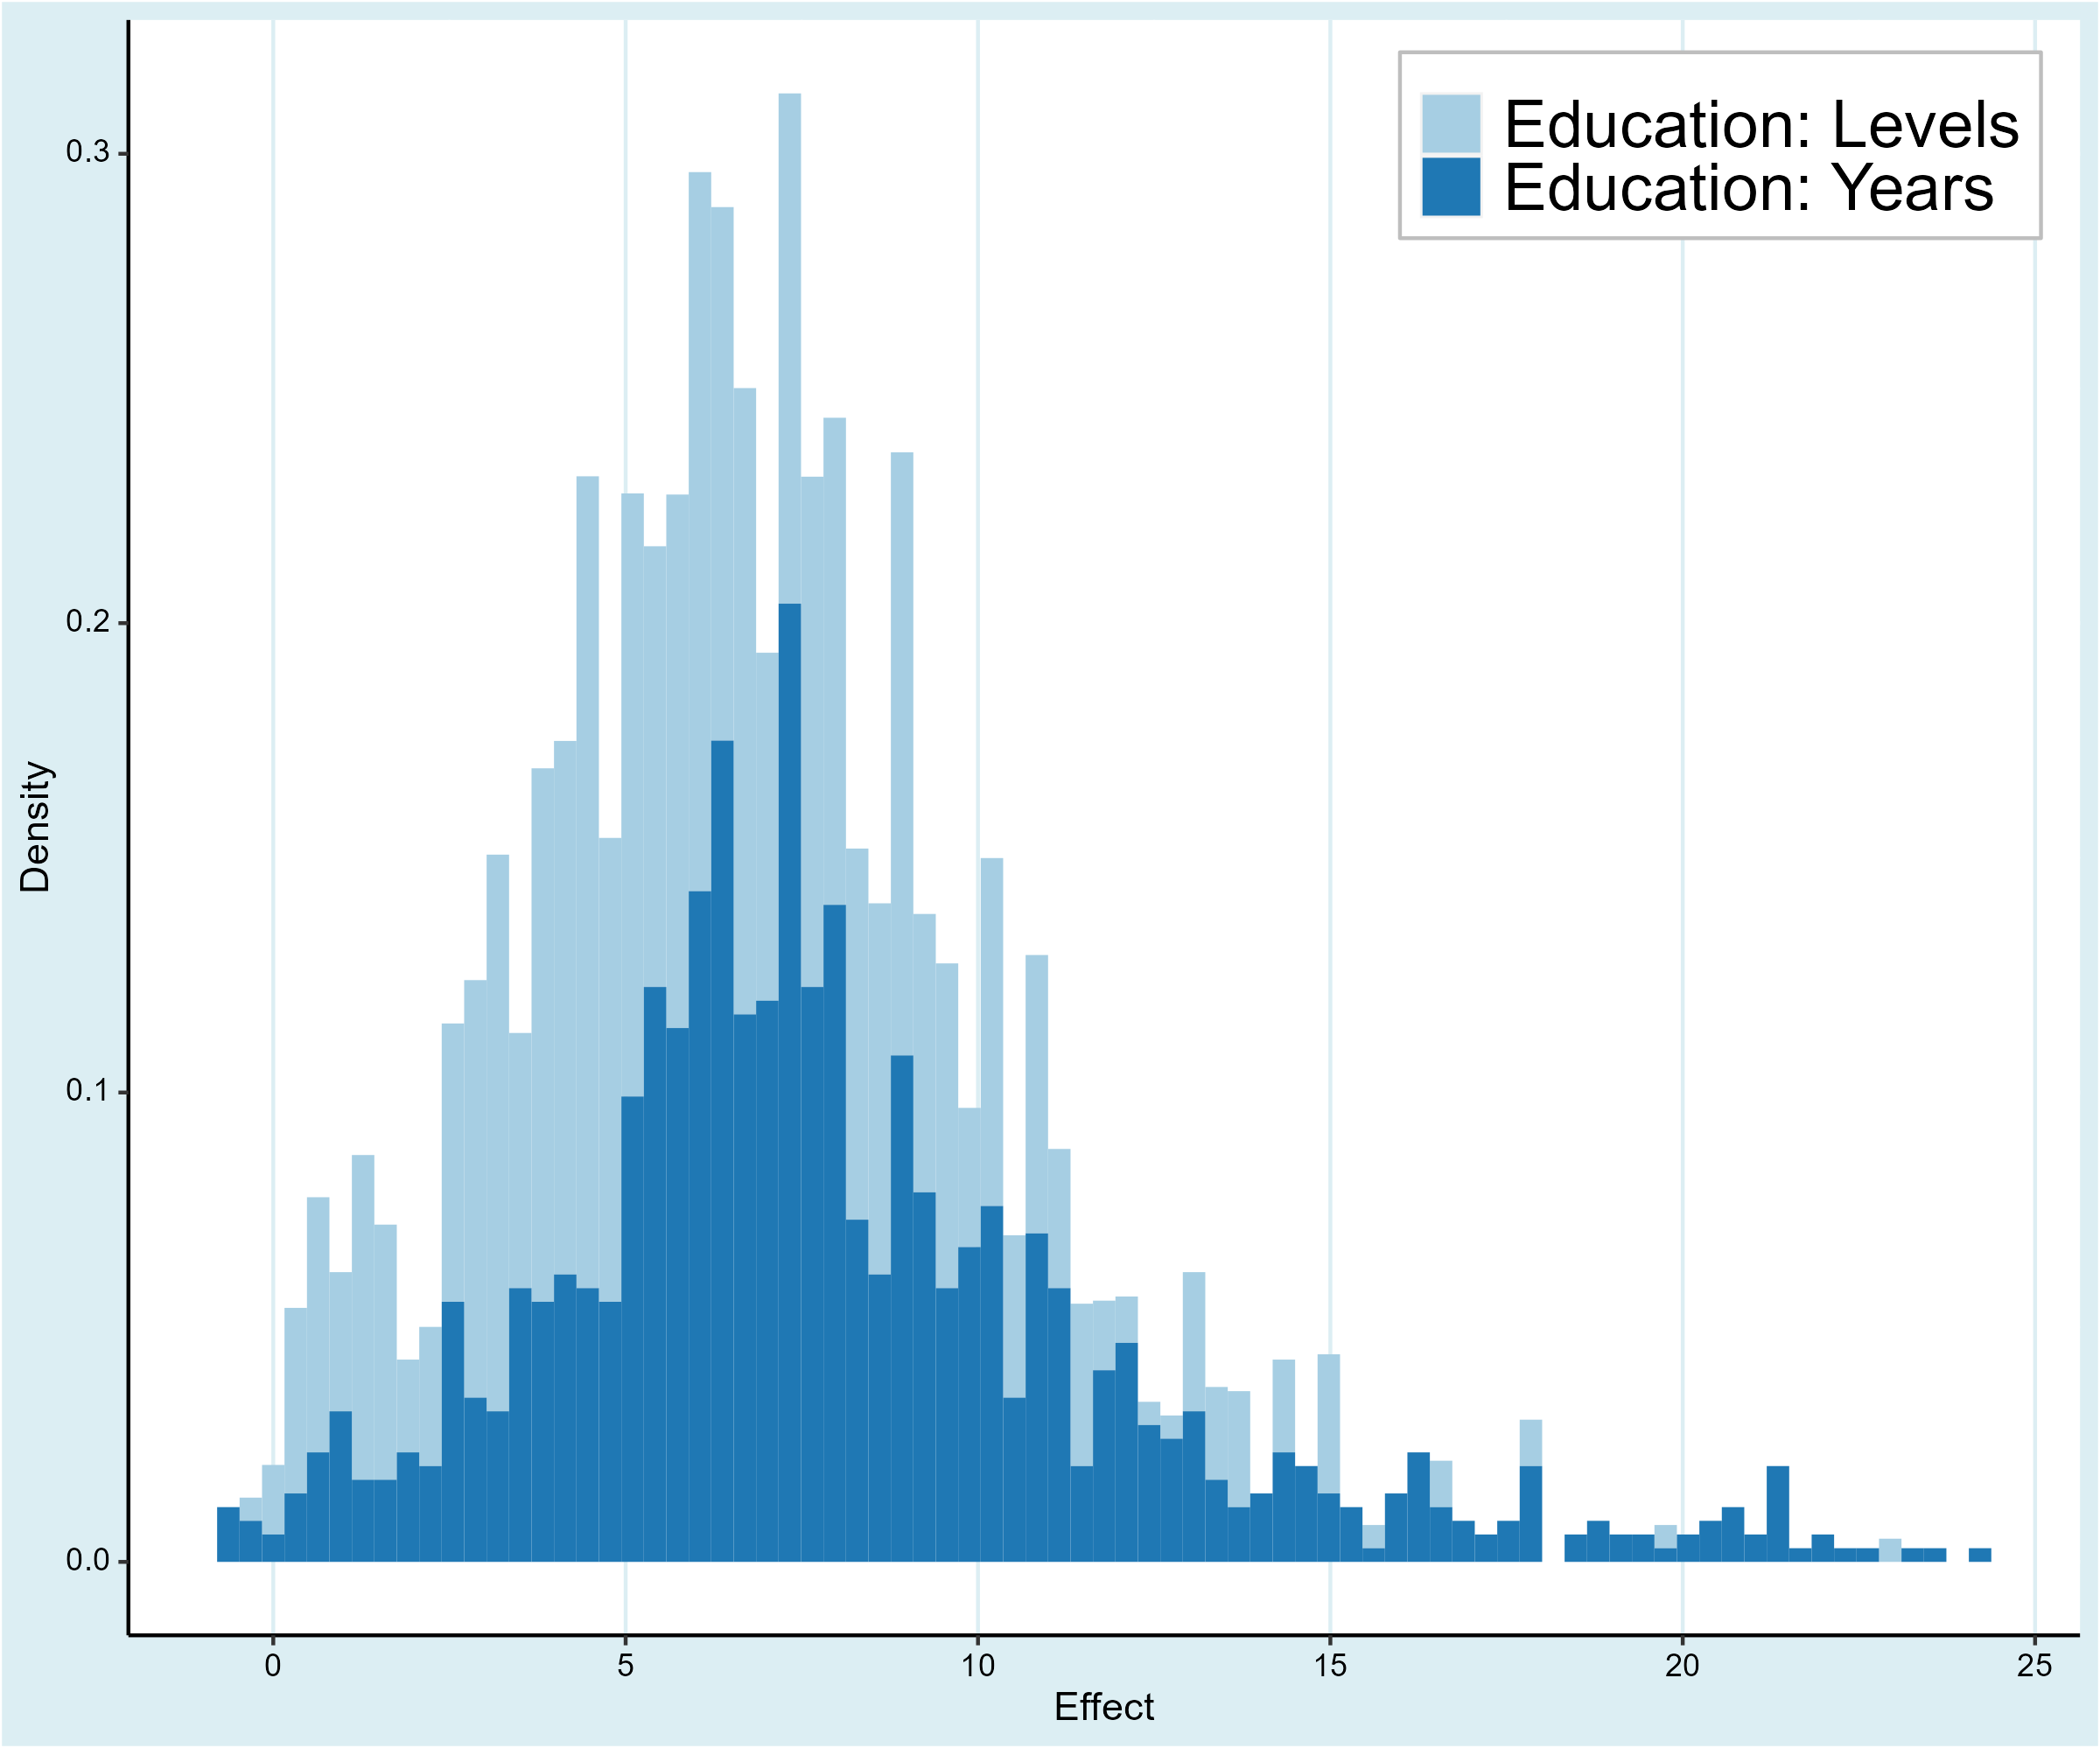
\includegraphics[width=0.95\linewidth]{Figures/Prima Facie/prima_facie_years_levels.png}
         \label{fig:prima_facie_years_levels}
      \end{subfigure}
      \begin{subfigure}[!htbp]{0.38\textwidth}
         \vspace{-0.1cm}
         \caption{Data type}
         \vspace{-0.1cm}
         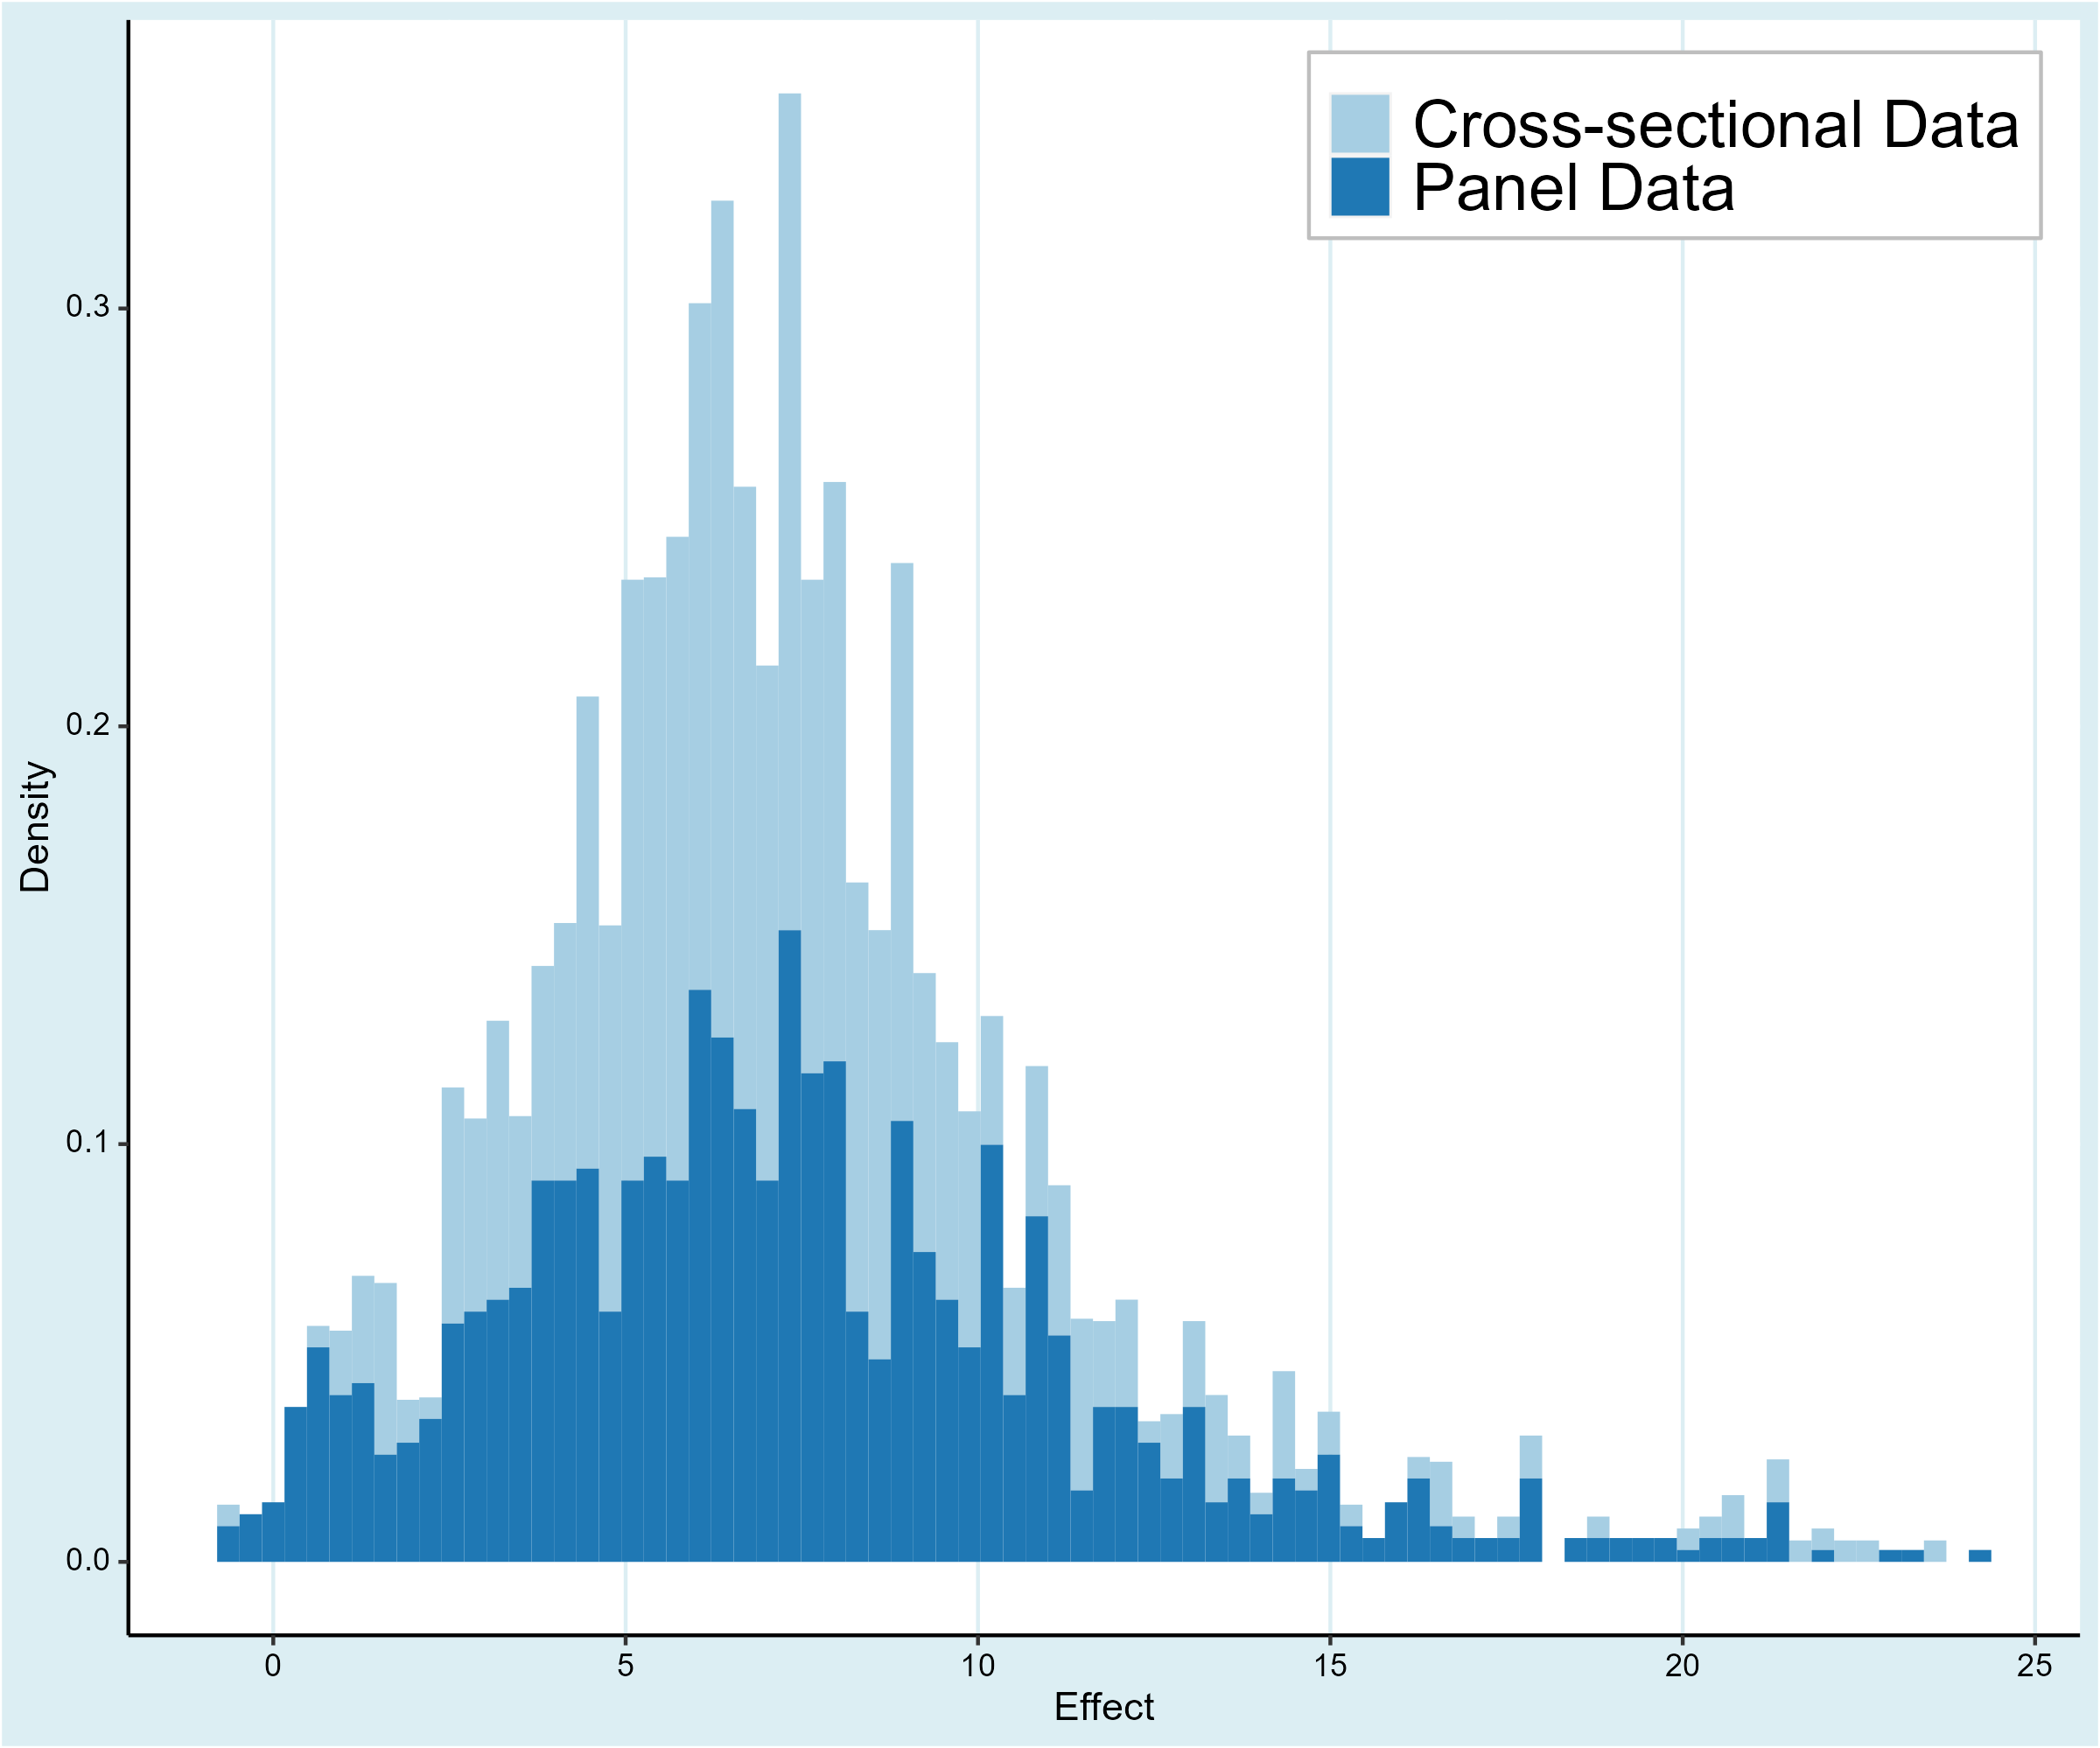
\includegraphics[width=0.95\linewidth]{Figures/Prima Facie/prima_facie_data_type.png}
         \label{fig:prima_facie_data_type}
      \end{subfigure}

      \begin{subfigure}[!htbp]{0.38\textwidth}
         \vspace{0.2cm}
         \caption{Highest education}
         \vspace{-0.1cm}
         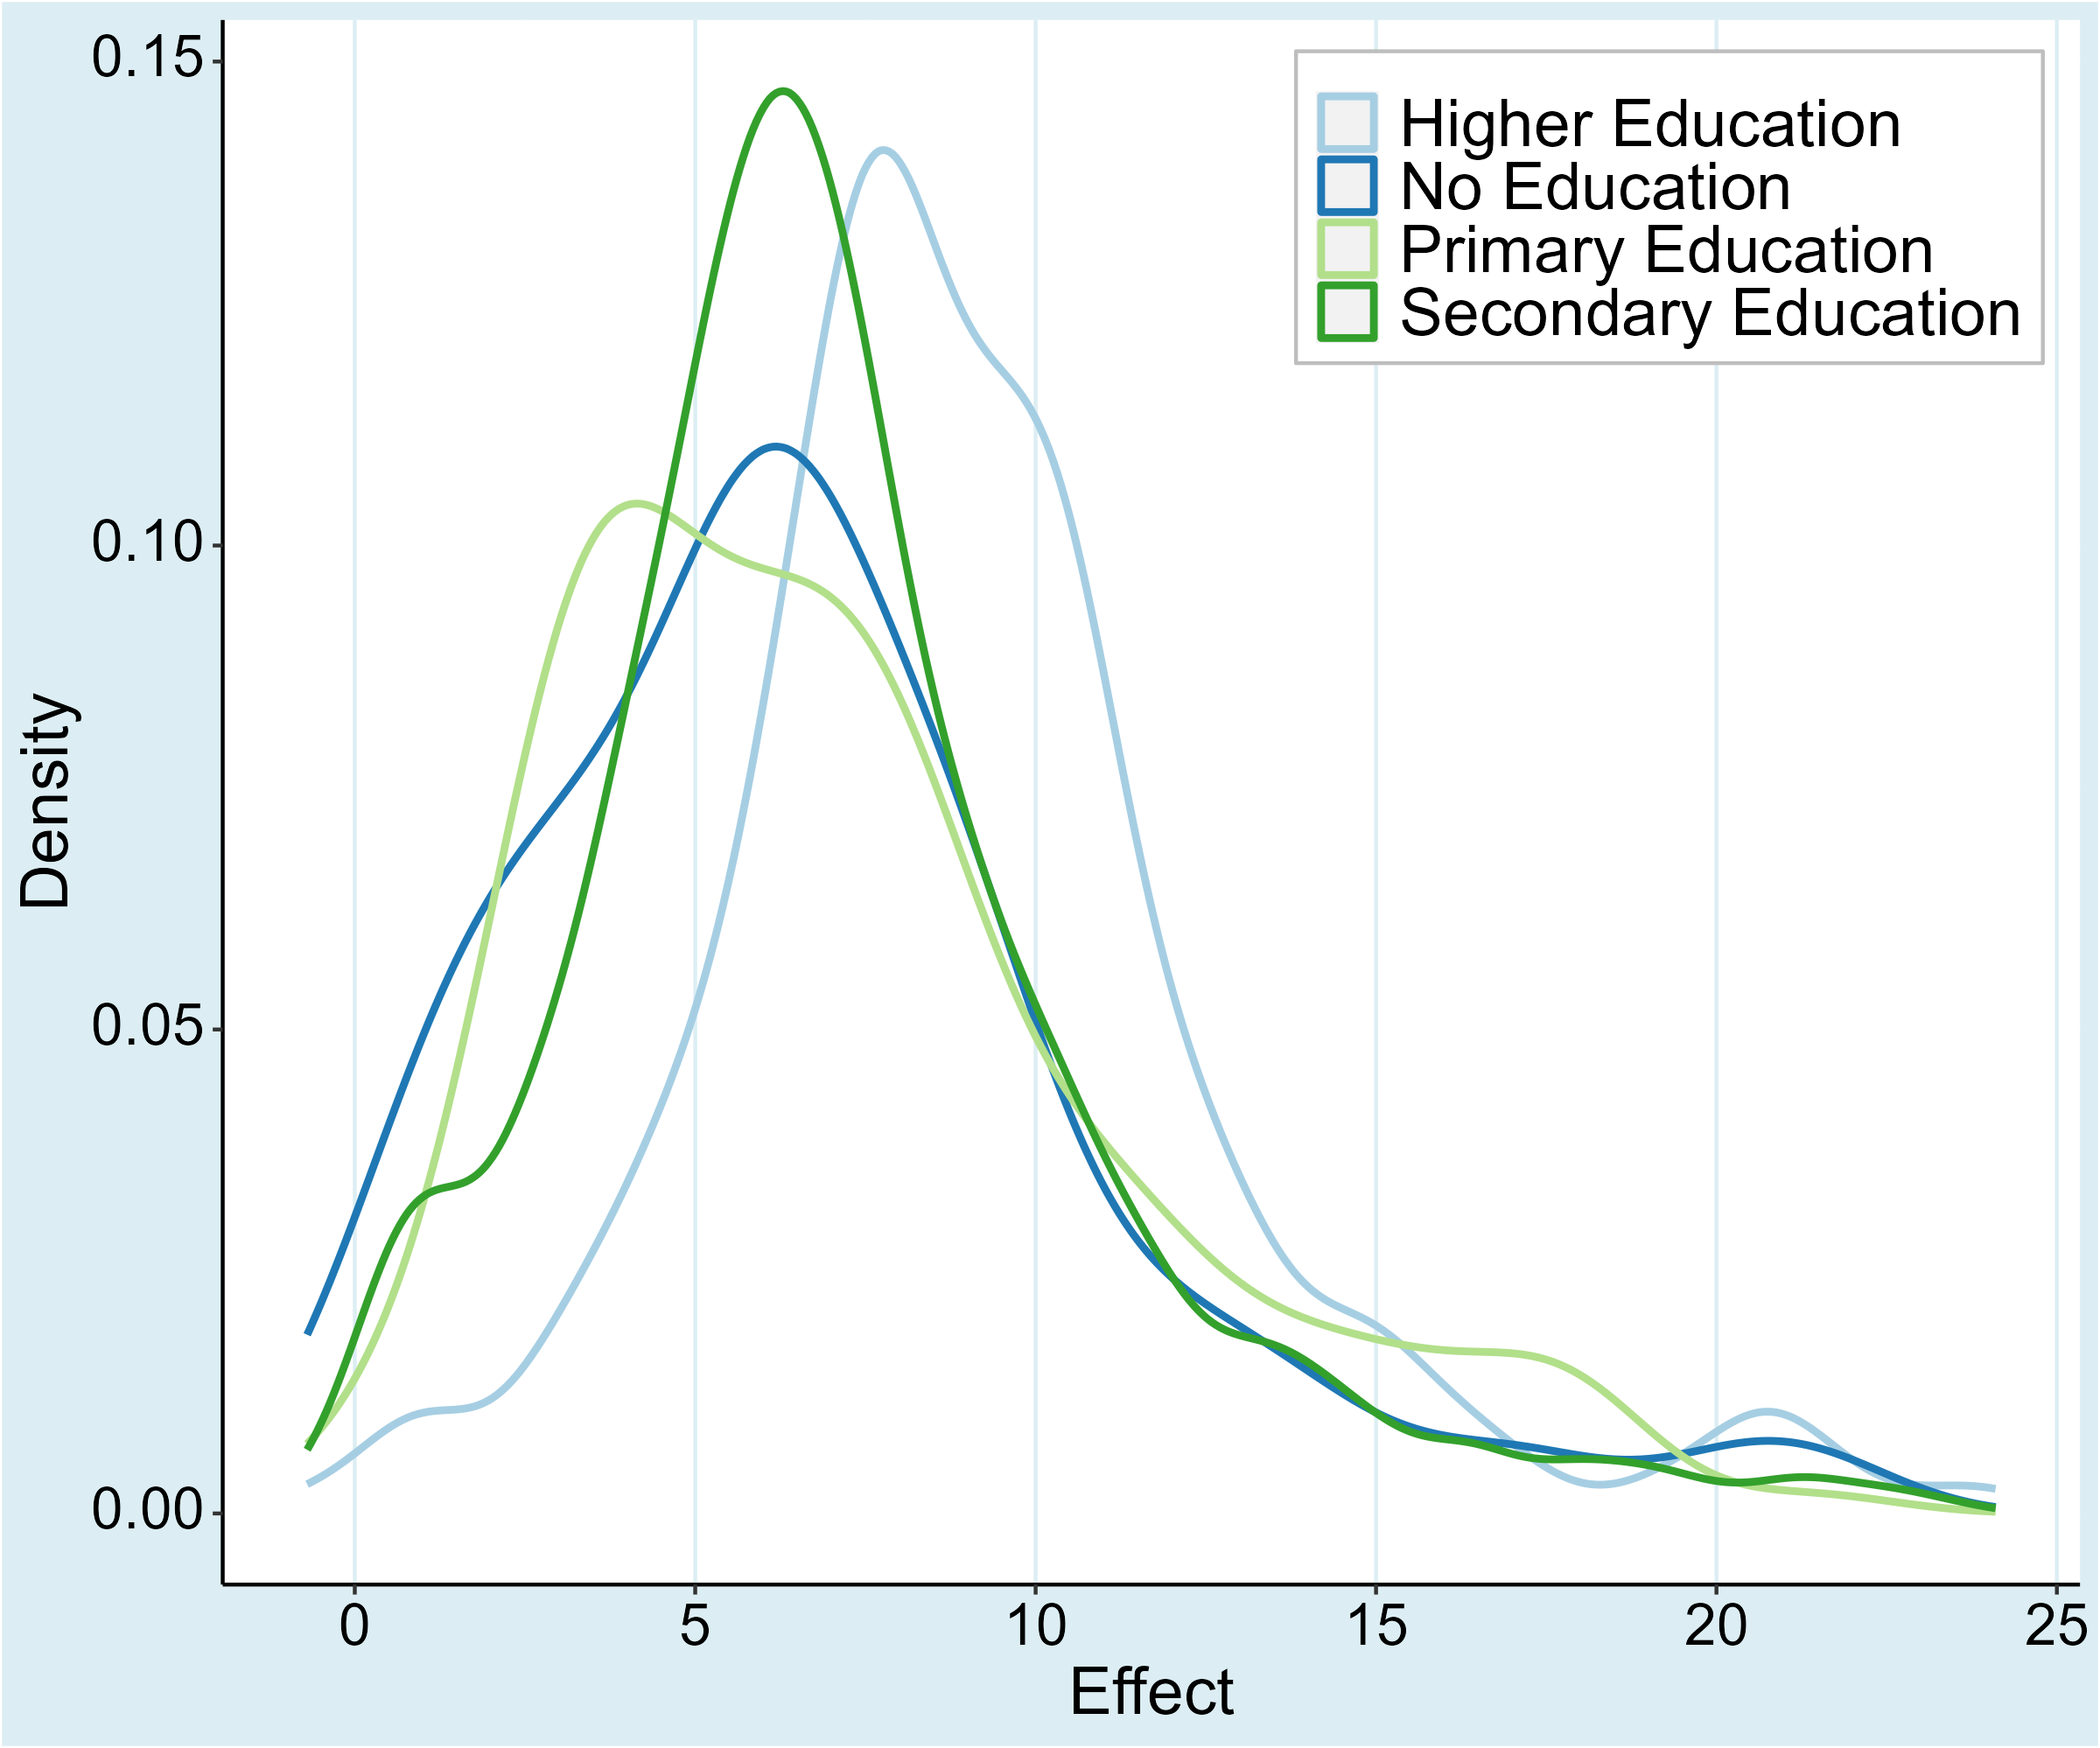
\includegraphics[width=0.95\linewidth]{Figures/Prima Facie/prima_facie_education.png}
         \label{fig:prima_facie_education}
      \end{subfigure}
      \begin{subfigure}[!htbp]{0.38\textwidth}
         \vspace{0.2cm}
         \caption{Gender}
         \vspace{-0.1cm}
         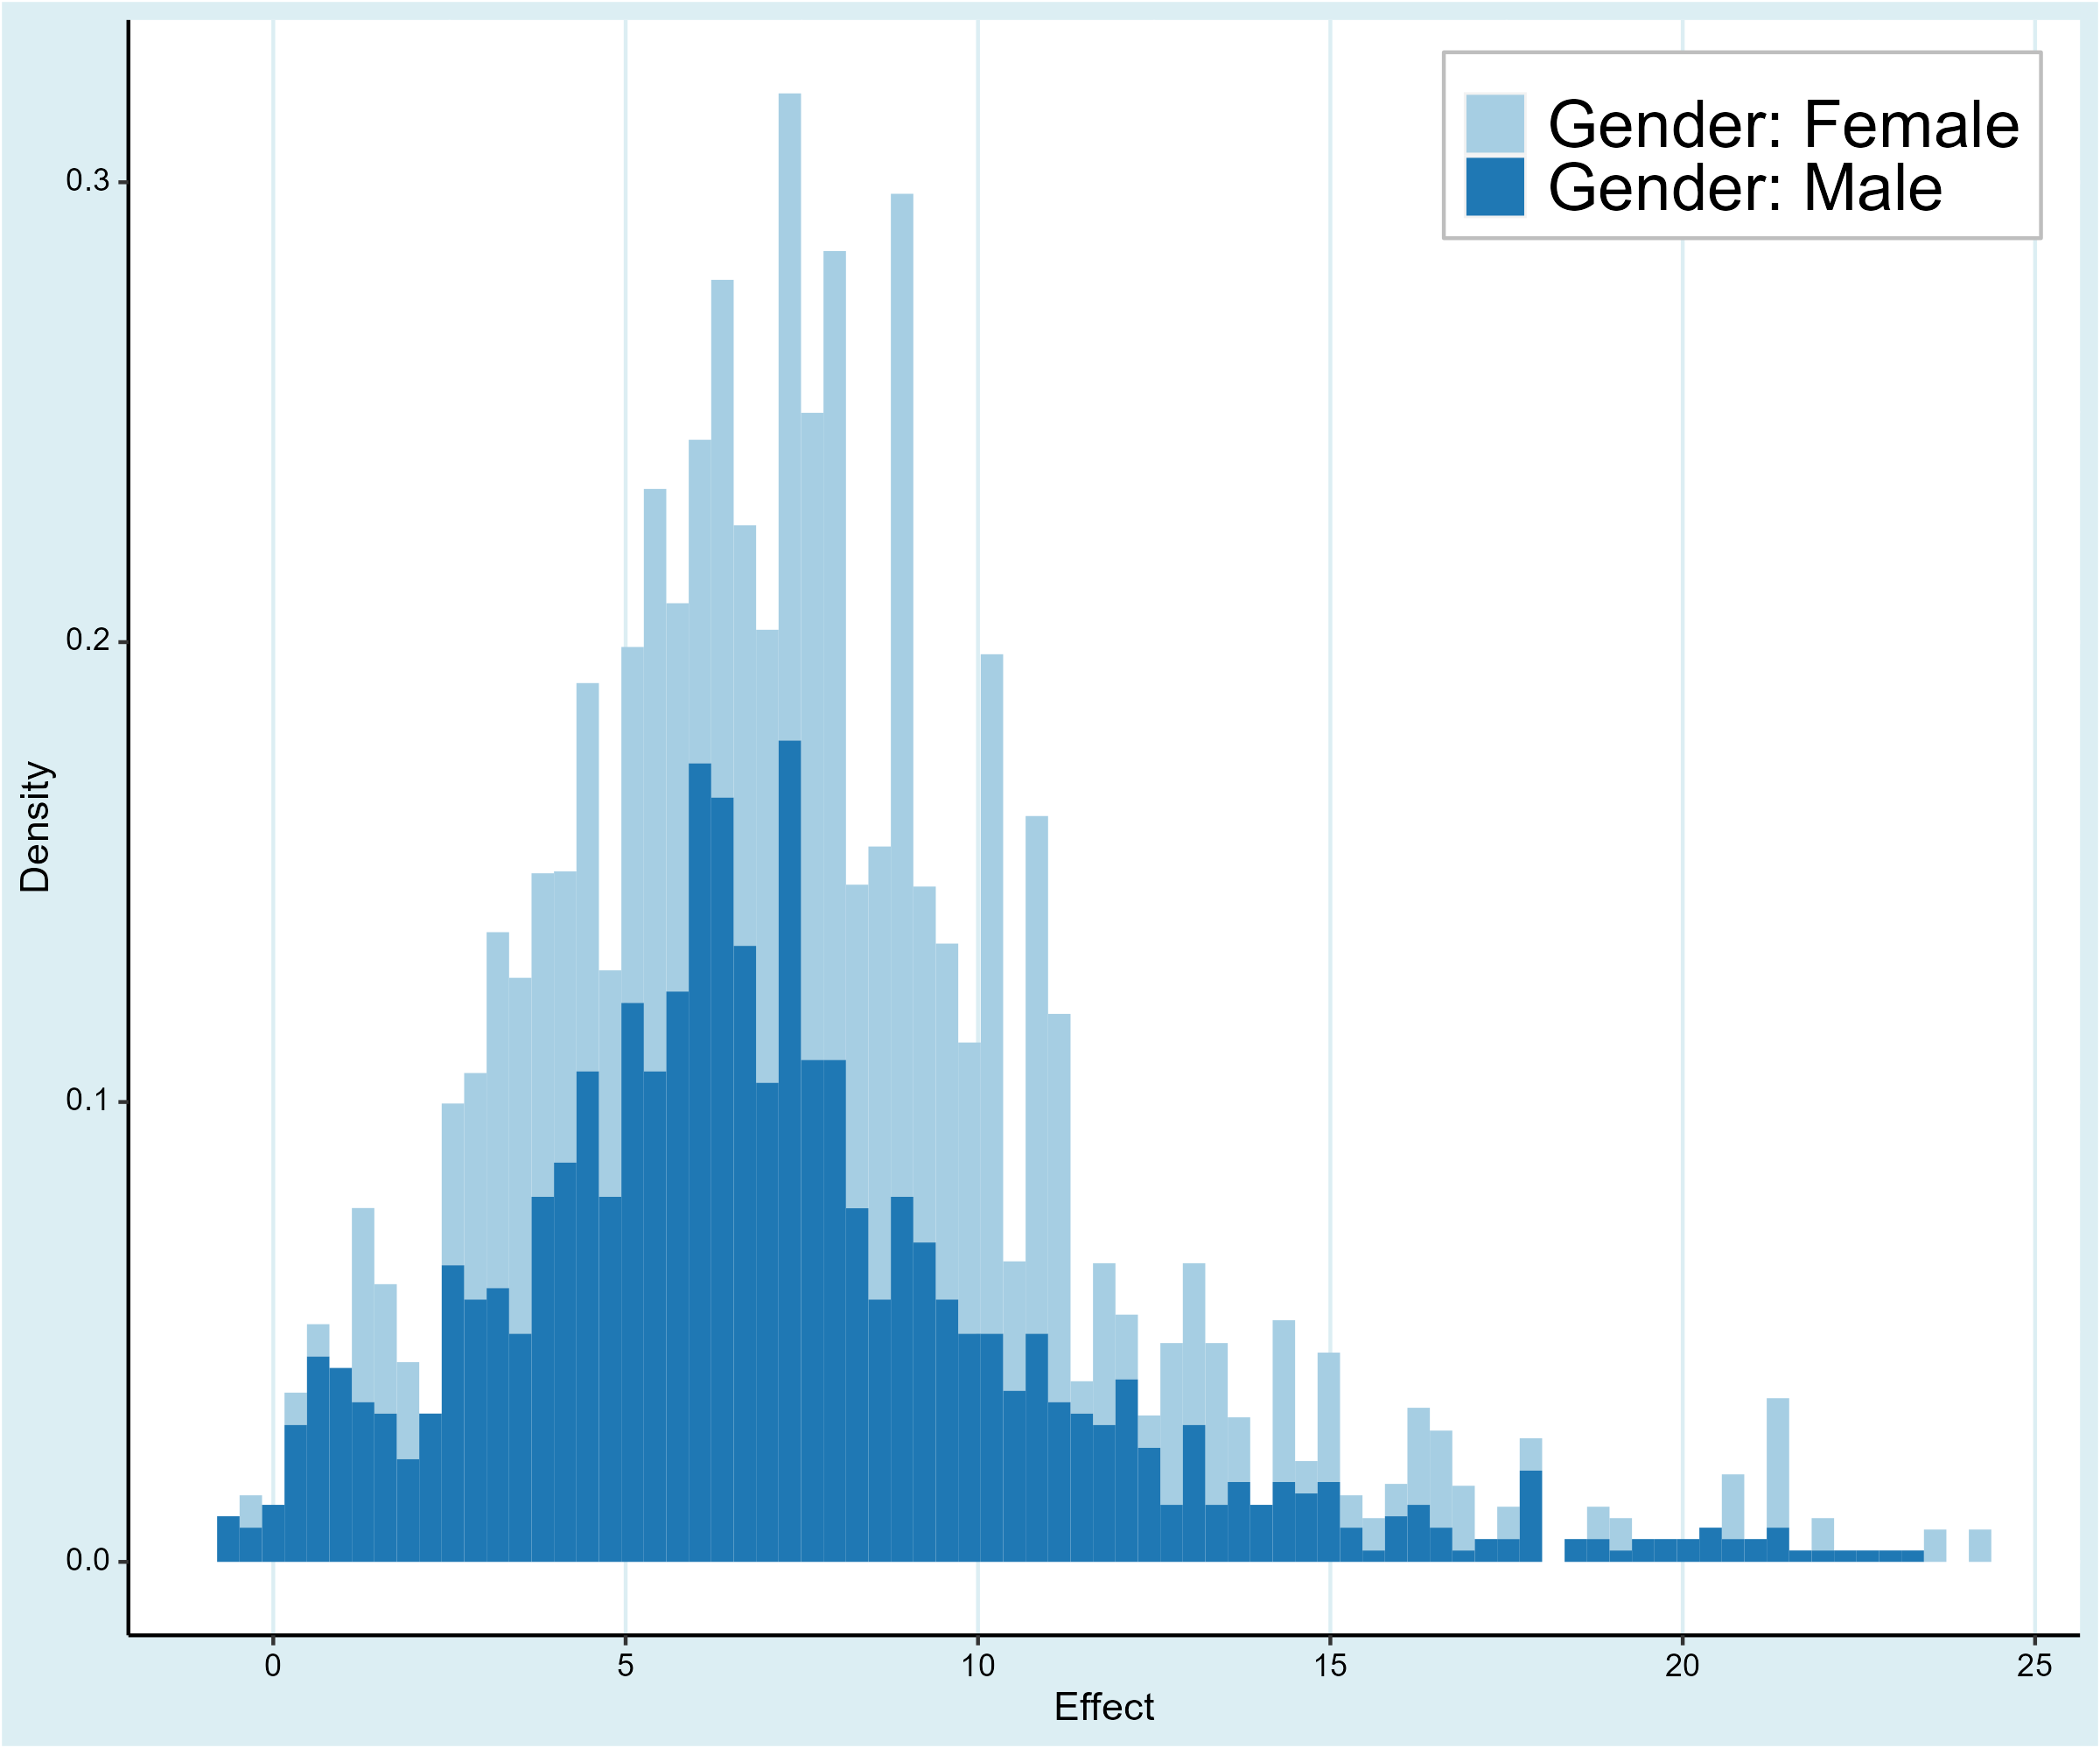
\includegraphics[width=0.95\linewidth]{Figures/Prima Facie/prima_facie_gender.png}
         \label{fig:prima_facie_gender}
      \end{subfigure}

      \begin{subfigure}[!htbp]{0.38\textwidth}
         \vspace{0.2cm}
         \caption{Country wealth}
         \vspace{-0.1cm}
         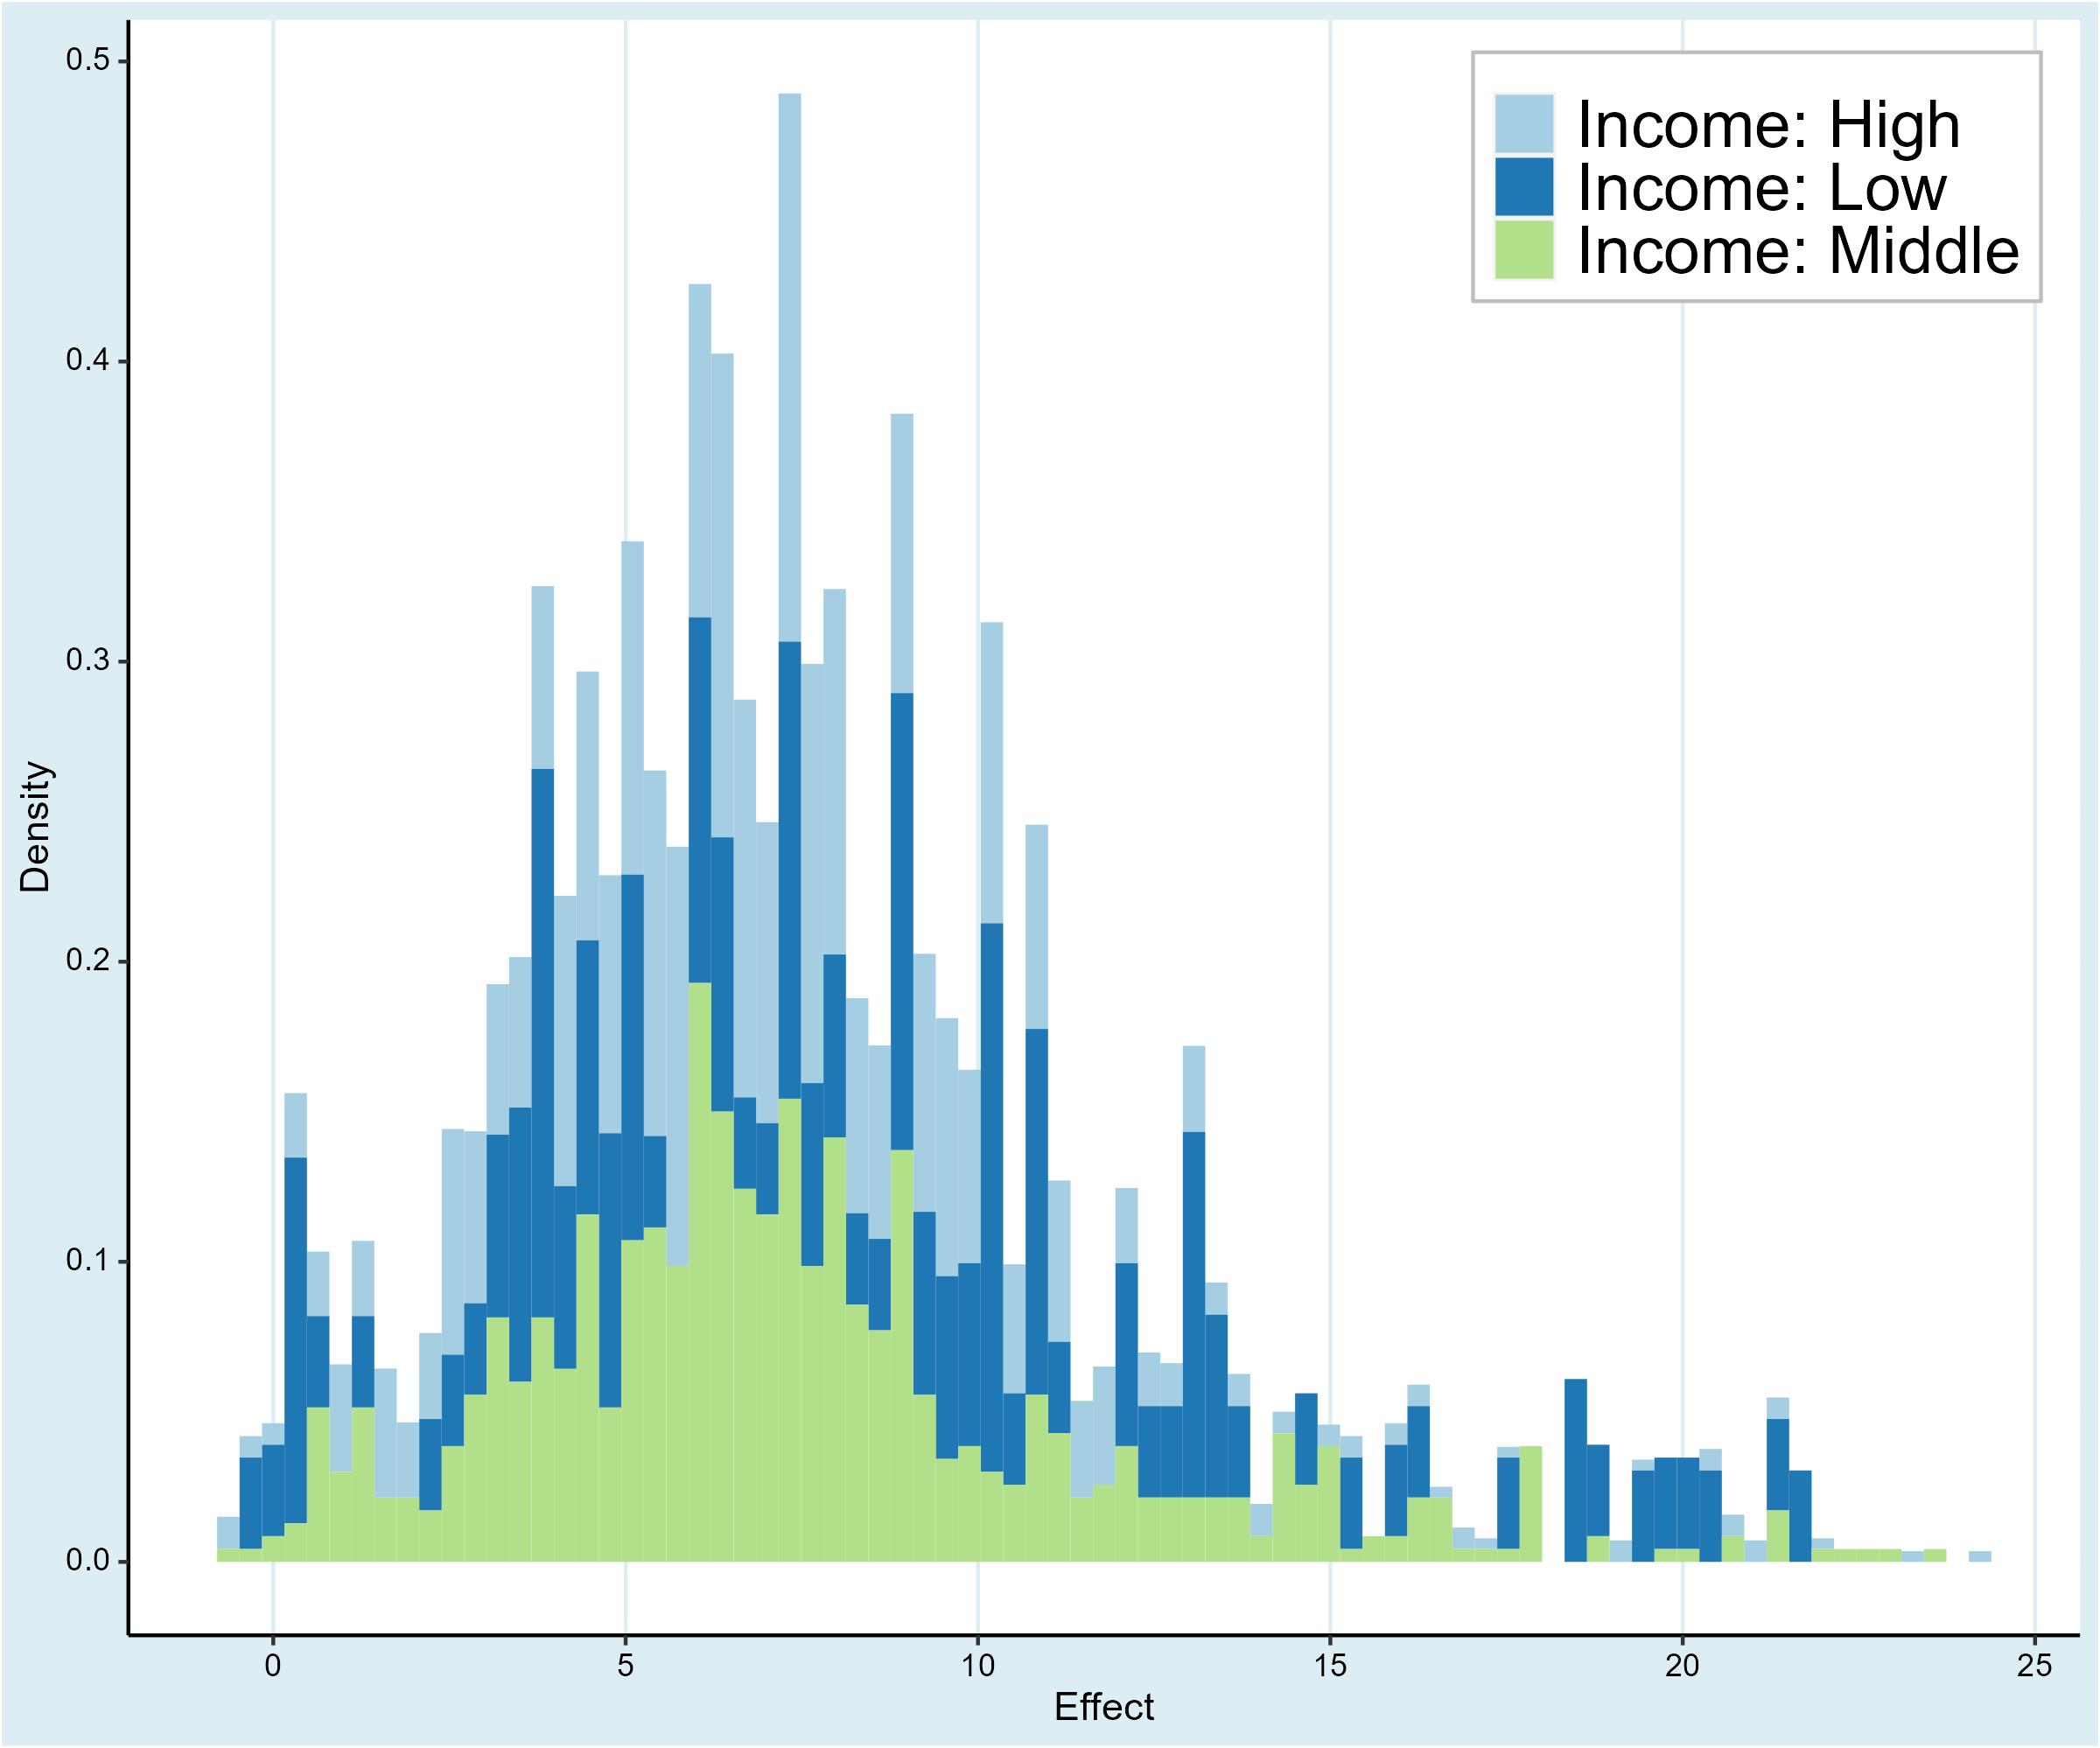
\includegraphics[width=0.95\linewidth]{Figures/Prima Facie/prima_facie_income.png}
         \label{fig:prima_facie_income}
      \end{subfigure}
      \begin{subfigure}[!htbp]{0.38\textwidth}
         \vspace{0.2cm}
         \caption{Estimation method}
         \vspace{-0.1cm}
         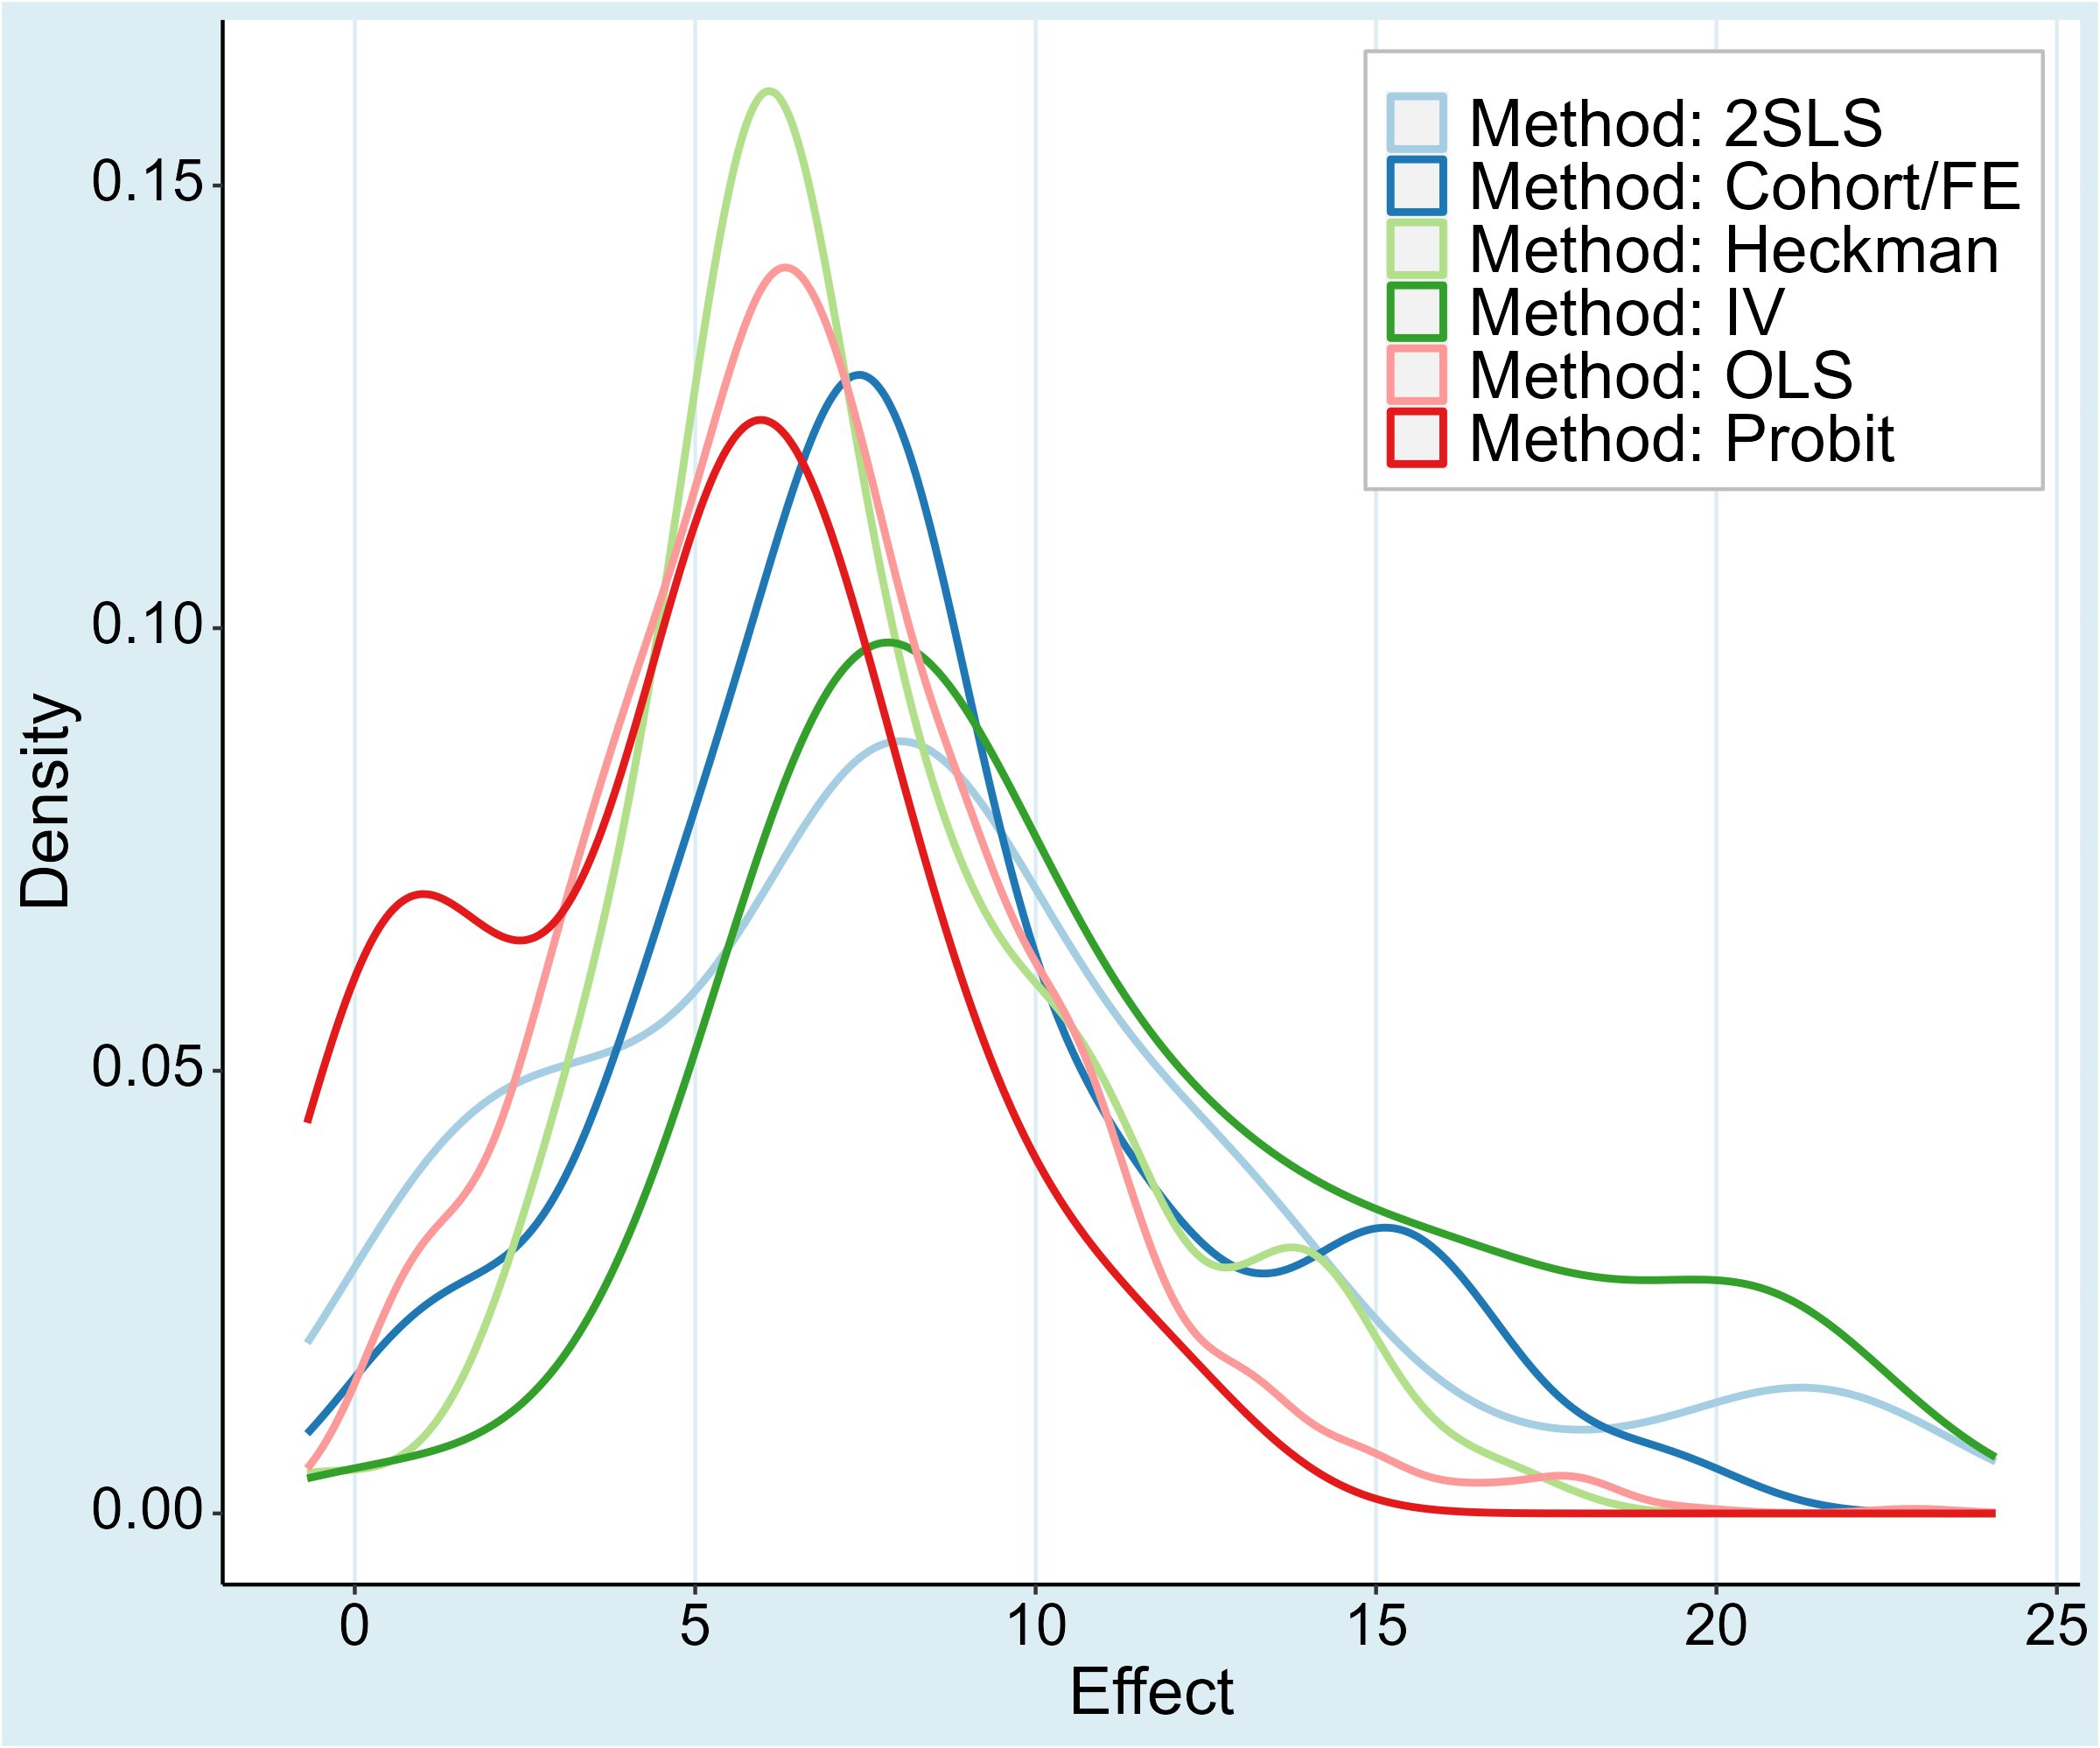
\includegraphics[width=0.95\linewidth]{Figures/Prima Facie/prima_facie_method.png}
         \label{fig:prima_facie_method}
      \end{subfigure}

      \begin{subfigure}[!htbp]{0.38\textwidth}
         \vspace{0.2cm}
         \caption{Ability}
         \vspace{-0.1cm}
         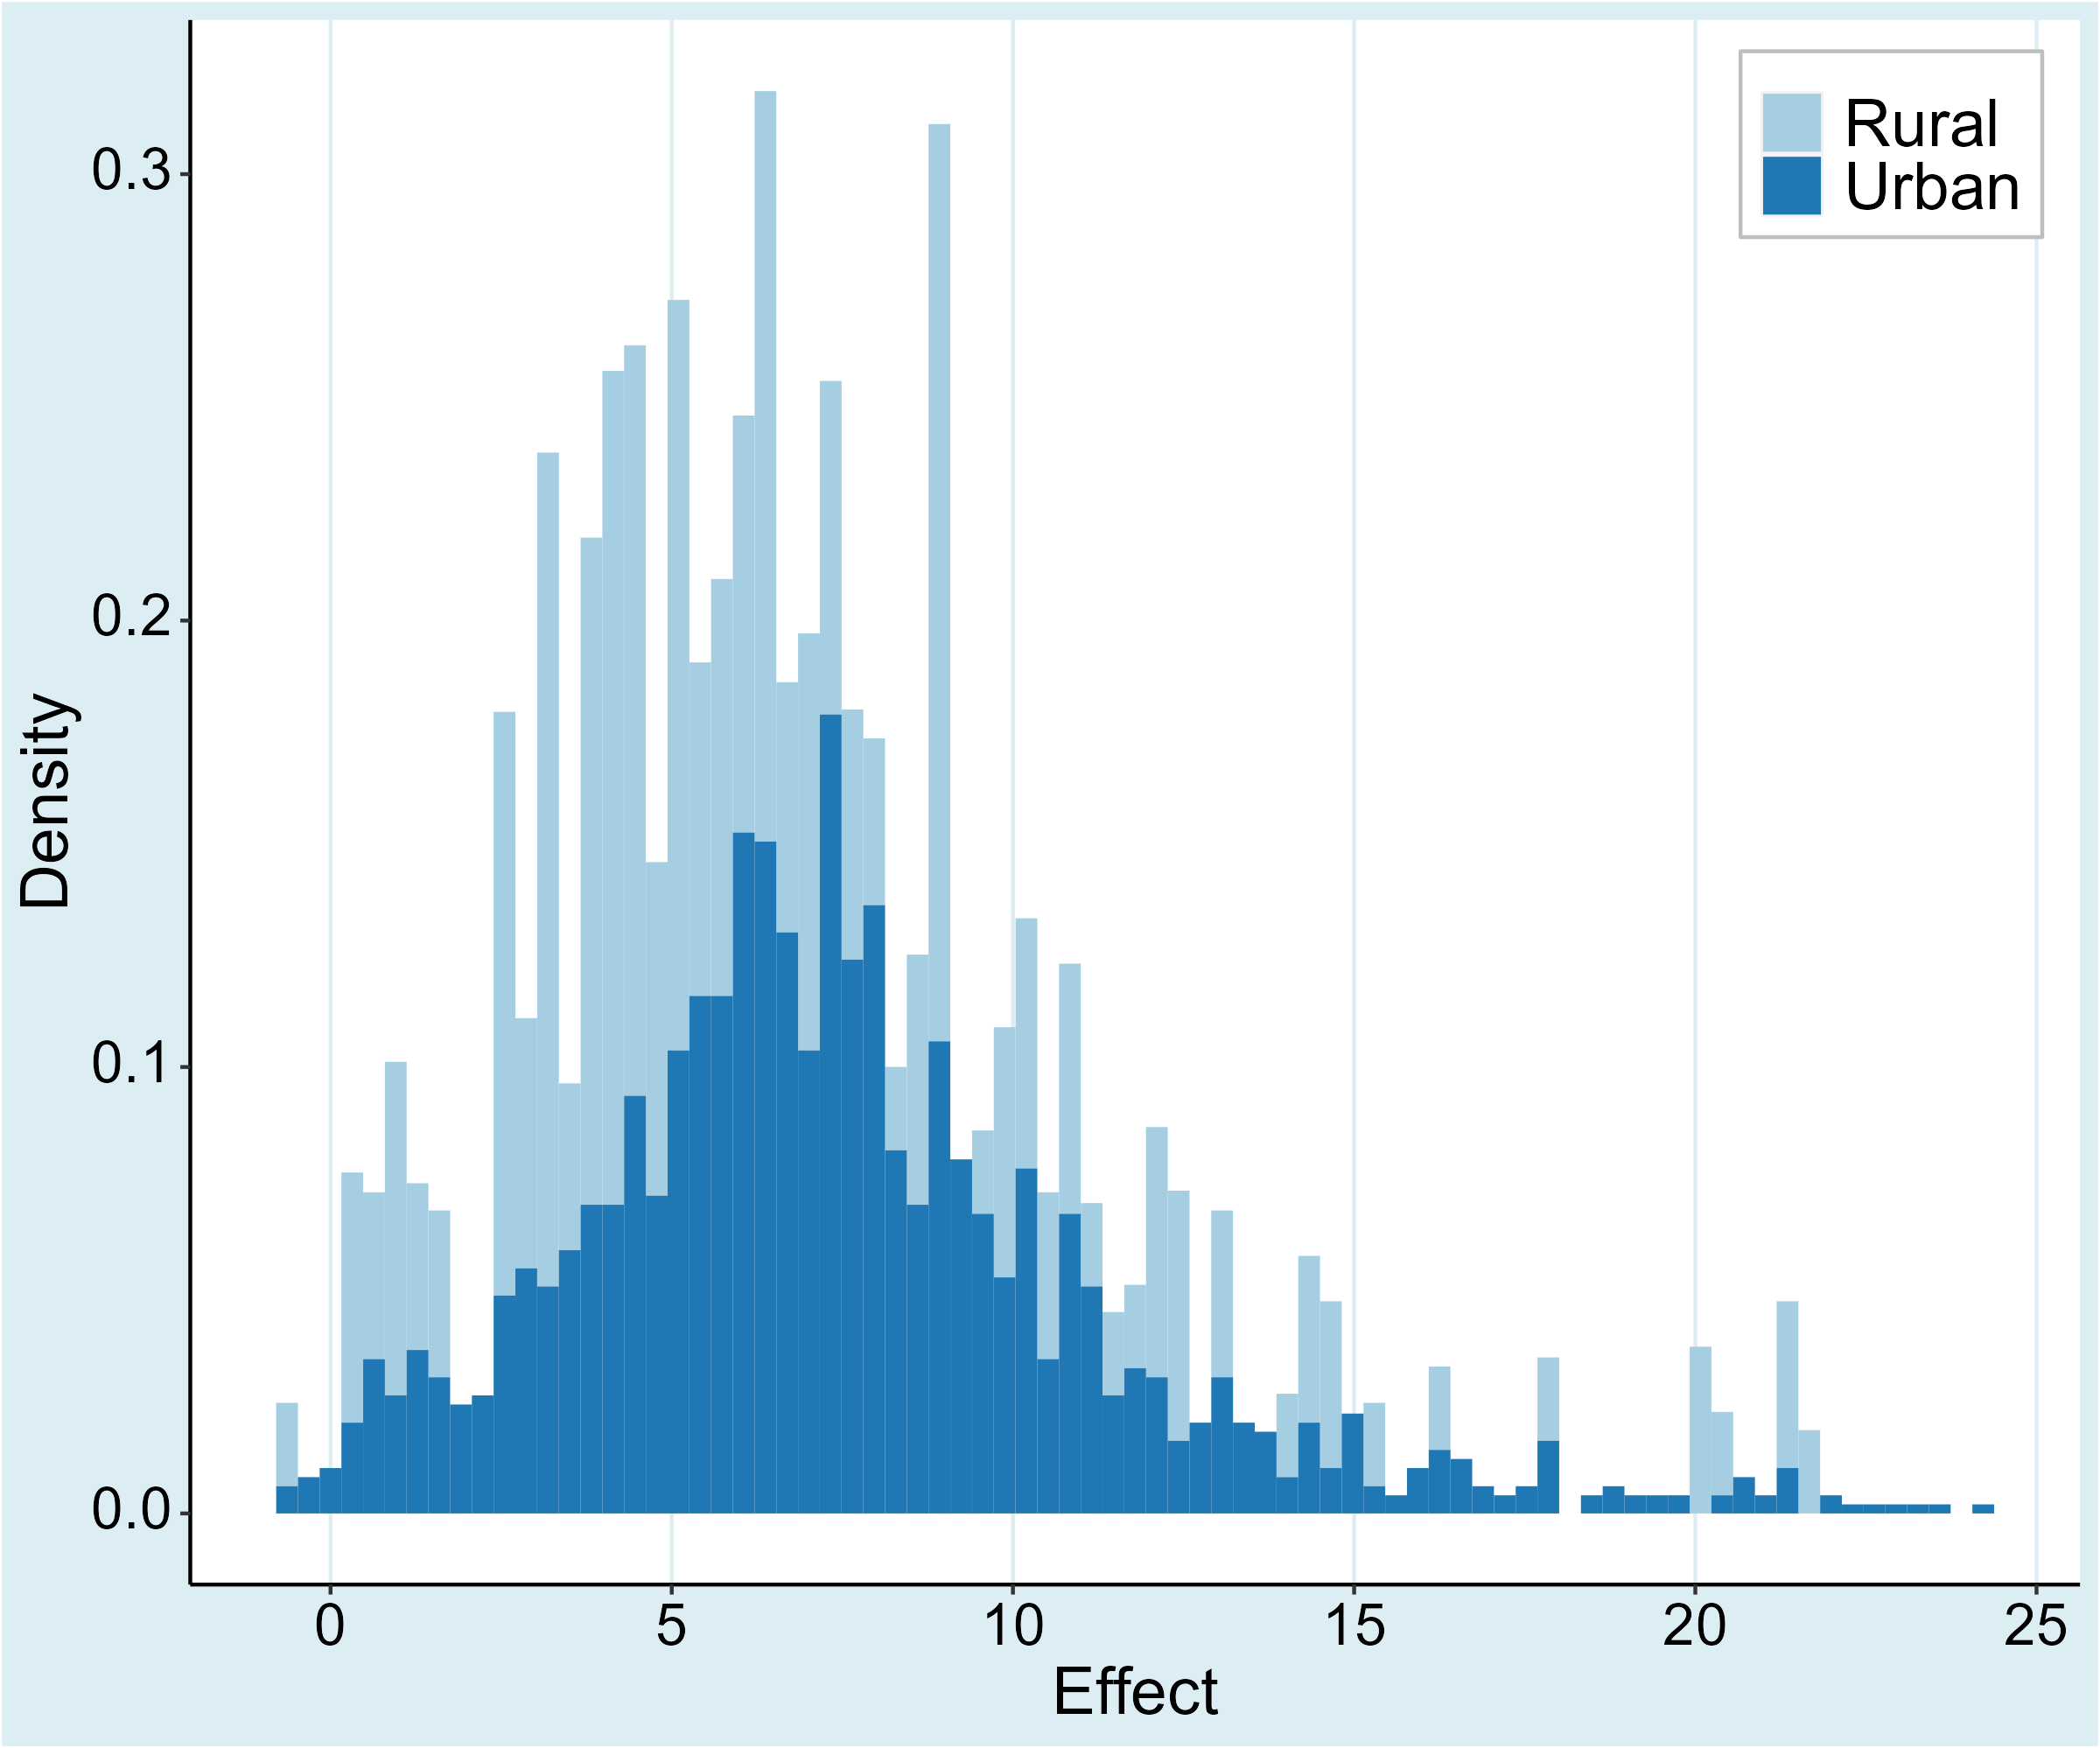
\includegraphics[width=0.95\linewidth]{Figures/Prima Facie/prima_facie_ability.png}
         \label{fig:prima_facie_ability}
      \end{subfigure}
      \begin{subfigure}[!htbp]{0.38\textwidth}
         \vspace{0.2cm}
         \caption{Citations}
         \vspace{-0.1cm}
         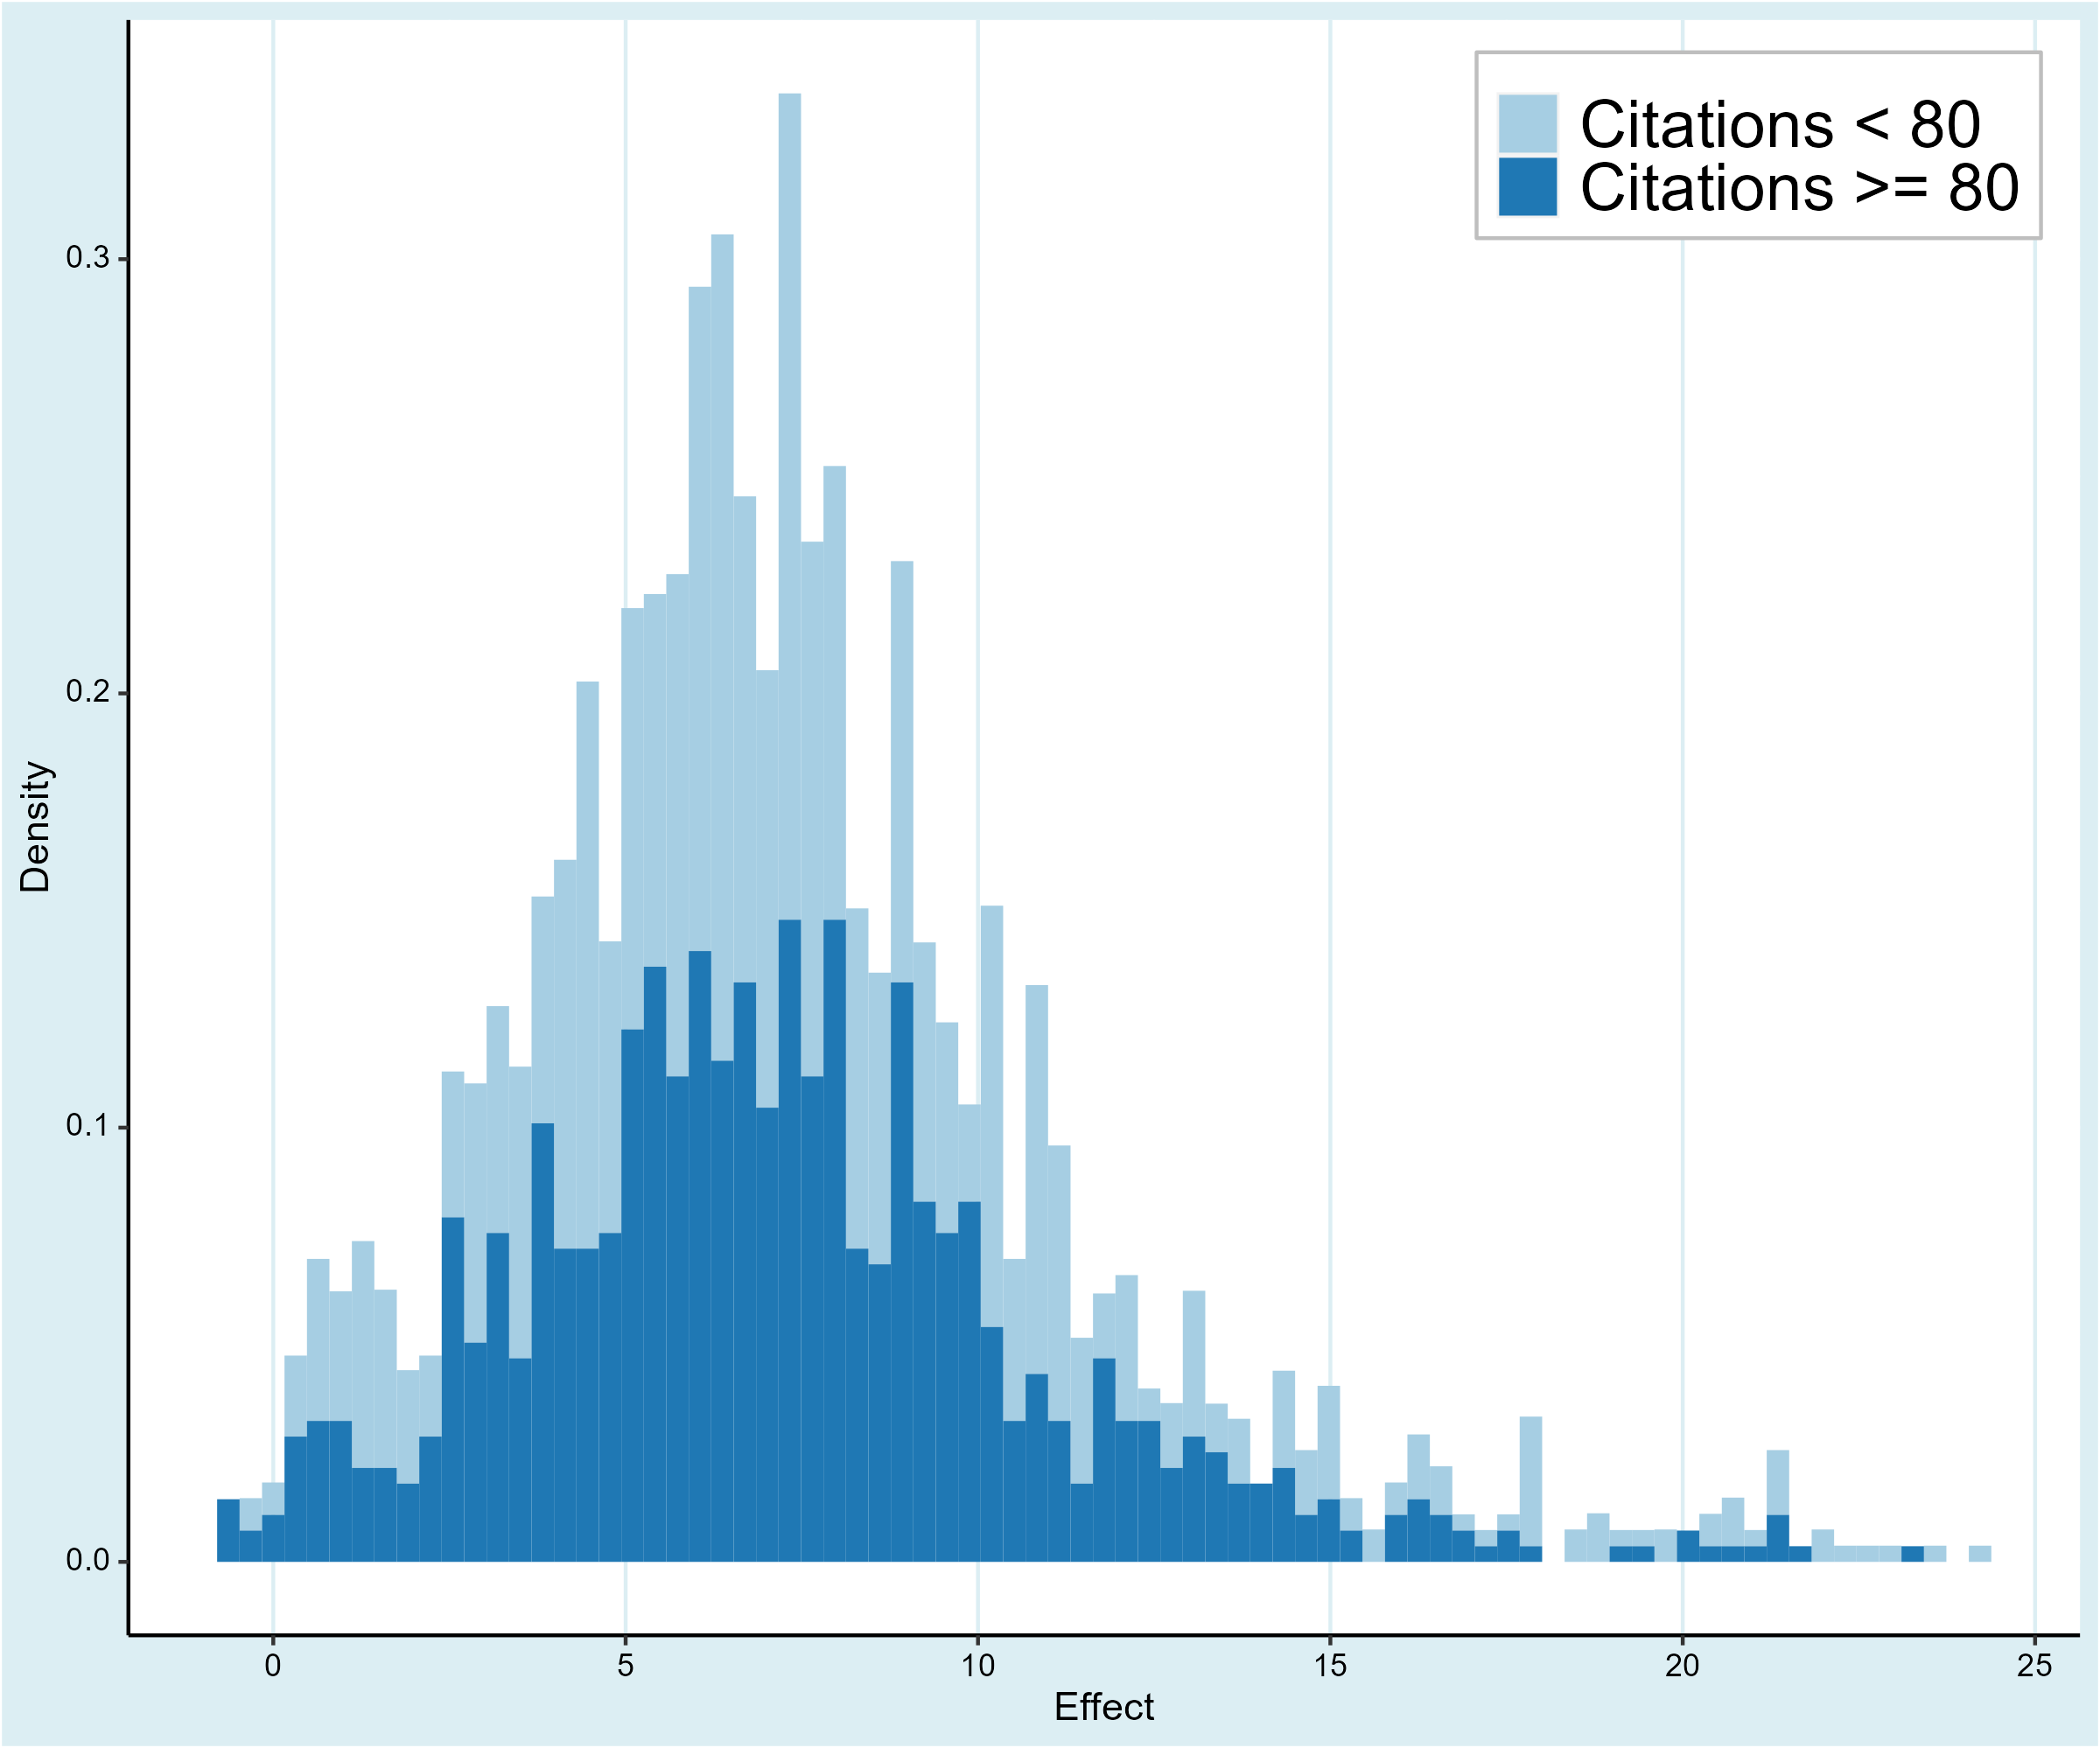
\includegraphics[width=0.95\linewidth]{Figures/Prima Facie/prima_facie_citations.png}
         \label{fig:prima_facie_citations}
      \end{subfigure}

   \end{center}\vspace{-0.6cm}
   \captionsetup{width=0.75\textwidth, font = scriptsize}
   \caption*{\emph{Note:} This figure displays histograms and density lines for different subsets of data, where the effect of an additional year of schooling on returns is displayed on the x-axis against its density on the y-axis. For \autoref{fig:prima_facie_citations}, the data median is used to determine the subsets. For a description of variables used in this figure, see \autoref{tab:var}.}
\end{figure}


Allow me now to I quickly address the numeric results. As a baseline for the rest of the work, we can observe that the unweighted mean of the effect across all data equals 7.476 (7.674 for the data weighted by the number of estimates reported per study). As a reminder, this can be interpreted as a 7.456\% increase in log wage per additional year of attained schooling and falls well into the expected range, comparing this estimate to the results of other works. As such, this brief insight can serve as a sanity check that there is nothing immediately wrong with the data collection. When comparing to individual studies, this mean is slightly lower than \cite{psacharopoulos2018meta} who claim about 9\% average returns to schooling, but a bit higher than the findings of \cite{fleisher2005meta} who report returns between 5 and 6 percent on average. My results also align well with the only study dealing in detail with ability bias, \cite{wincenciak2022meta}, where the authors also report a 7\% figure for the average effect. Note that the suggested figure of 7.476 does not account for publication bias and should thus be treated only as a benchmark for further comparisons.

Concerning other subsets of data, there appears to be variety in several variable categories, including the age of data, economic status of countries, study publication status, or, perhaps more interestingly, ability. Estimates aggregated on the city level can be associated with higher estimates of the effect (8.5\%), yet this difference disappears entirely after accounting for the study size (7.6\%). The same is true for estimates from unpublished studies (8.3\% vs. 7.7\%). On the other hand, estimates associated with other variables remain higher than their counterparts, even through weighting. These include smaller sample size estimates, smaller studies, newer data, estimates for subjects with higher education, countries with low income, female subjects, or studies with a smaller impact factor. Perhaps most interestingly, the mean estimate is also higher for studies that proxy for ability and marginally for those that do not control for it.

However, given the wide confidence intervals associated with all these subsets, one should take all these claims with a grain of salt. Furthermore, these differences are only marginal and should not serve as concrete evidence of a clear trend. Moreover, the mean could hardly be considered a statistical measure with perfect information; more data scrutiny will surely be necessary. This I will focus on in \autoref{chap:five}.

As for the graphical insights that can be obtained from the data, \autoref{fig:prima_facie_education} confirms that the distribution of estimates associated with higher education holds perhaps estimates of higher returns than its counterparts. Further, the right tail of the \textit{Ability: Proxied} variable distribution appears the heaviest out of the four subcategories. This may suggest that including a proxy for ability often yields higher estimates in ranges that other approaches seldom report. The right-side distribution tails also vary notably for the \textit{Method} variable, with \ac{IV} regression approach reporting the highest estimates of all techniques. In contrast, methods such as Probit or \ac{OLS} sporadically yield coefficients of unusually high value.

To highlight the differences between individual studies, I also include box plot of study-level clustered data in figures \ref{fig:box_plot_studies_1} and \ref{fig:box_plot_studies_2} (in the \autoref{app:one}, you may also find a country-level box plot for additional insight into the data). For clarity of presentation, I present two plots instead of one due to the large number of studies within the dataset. The split is done arbitrarily after 60 studies, ordered alphabetically. Despite the evident presence of outliers in some cases \citep{asadullah2006returns, harmon2002returns}, the studies, in most cases, report results close to the mean; only a handful of studies stand in the plot far out from the mean line. Studies of \cite{depken2019returns, girma2005heterogeneity}, or \cite{mphuka2012estimating} report peculiarly high estimates, while studies like \cite{angrist1995economic, li2007effect}, or \cite{webbink2004returns} never report an estimate above 5\% according to my calculations. To detect and amend for any potential miscalculations and human error, I double-checked the source data along with the calculations and, after this validation, proclaimed the dataset as final.

\afterpage{
   \begin{figure}[!t]
      \begin{center}
         \caption{Box plot of estimates across individual studies - first part}
         \label{fig:box_plot_studies_1}
         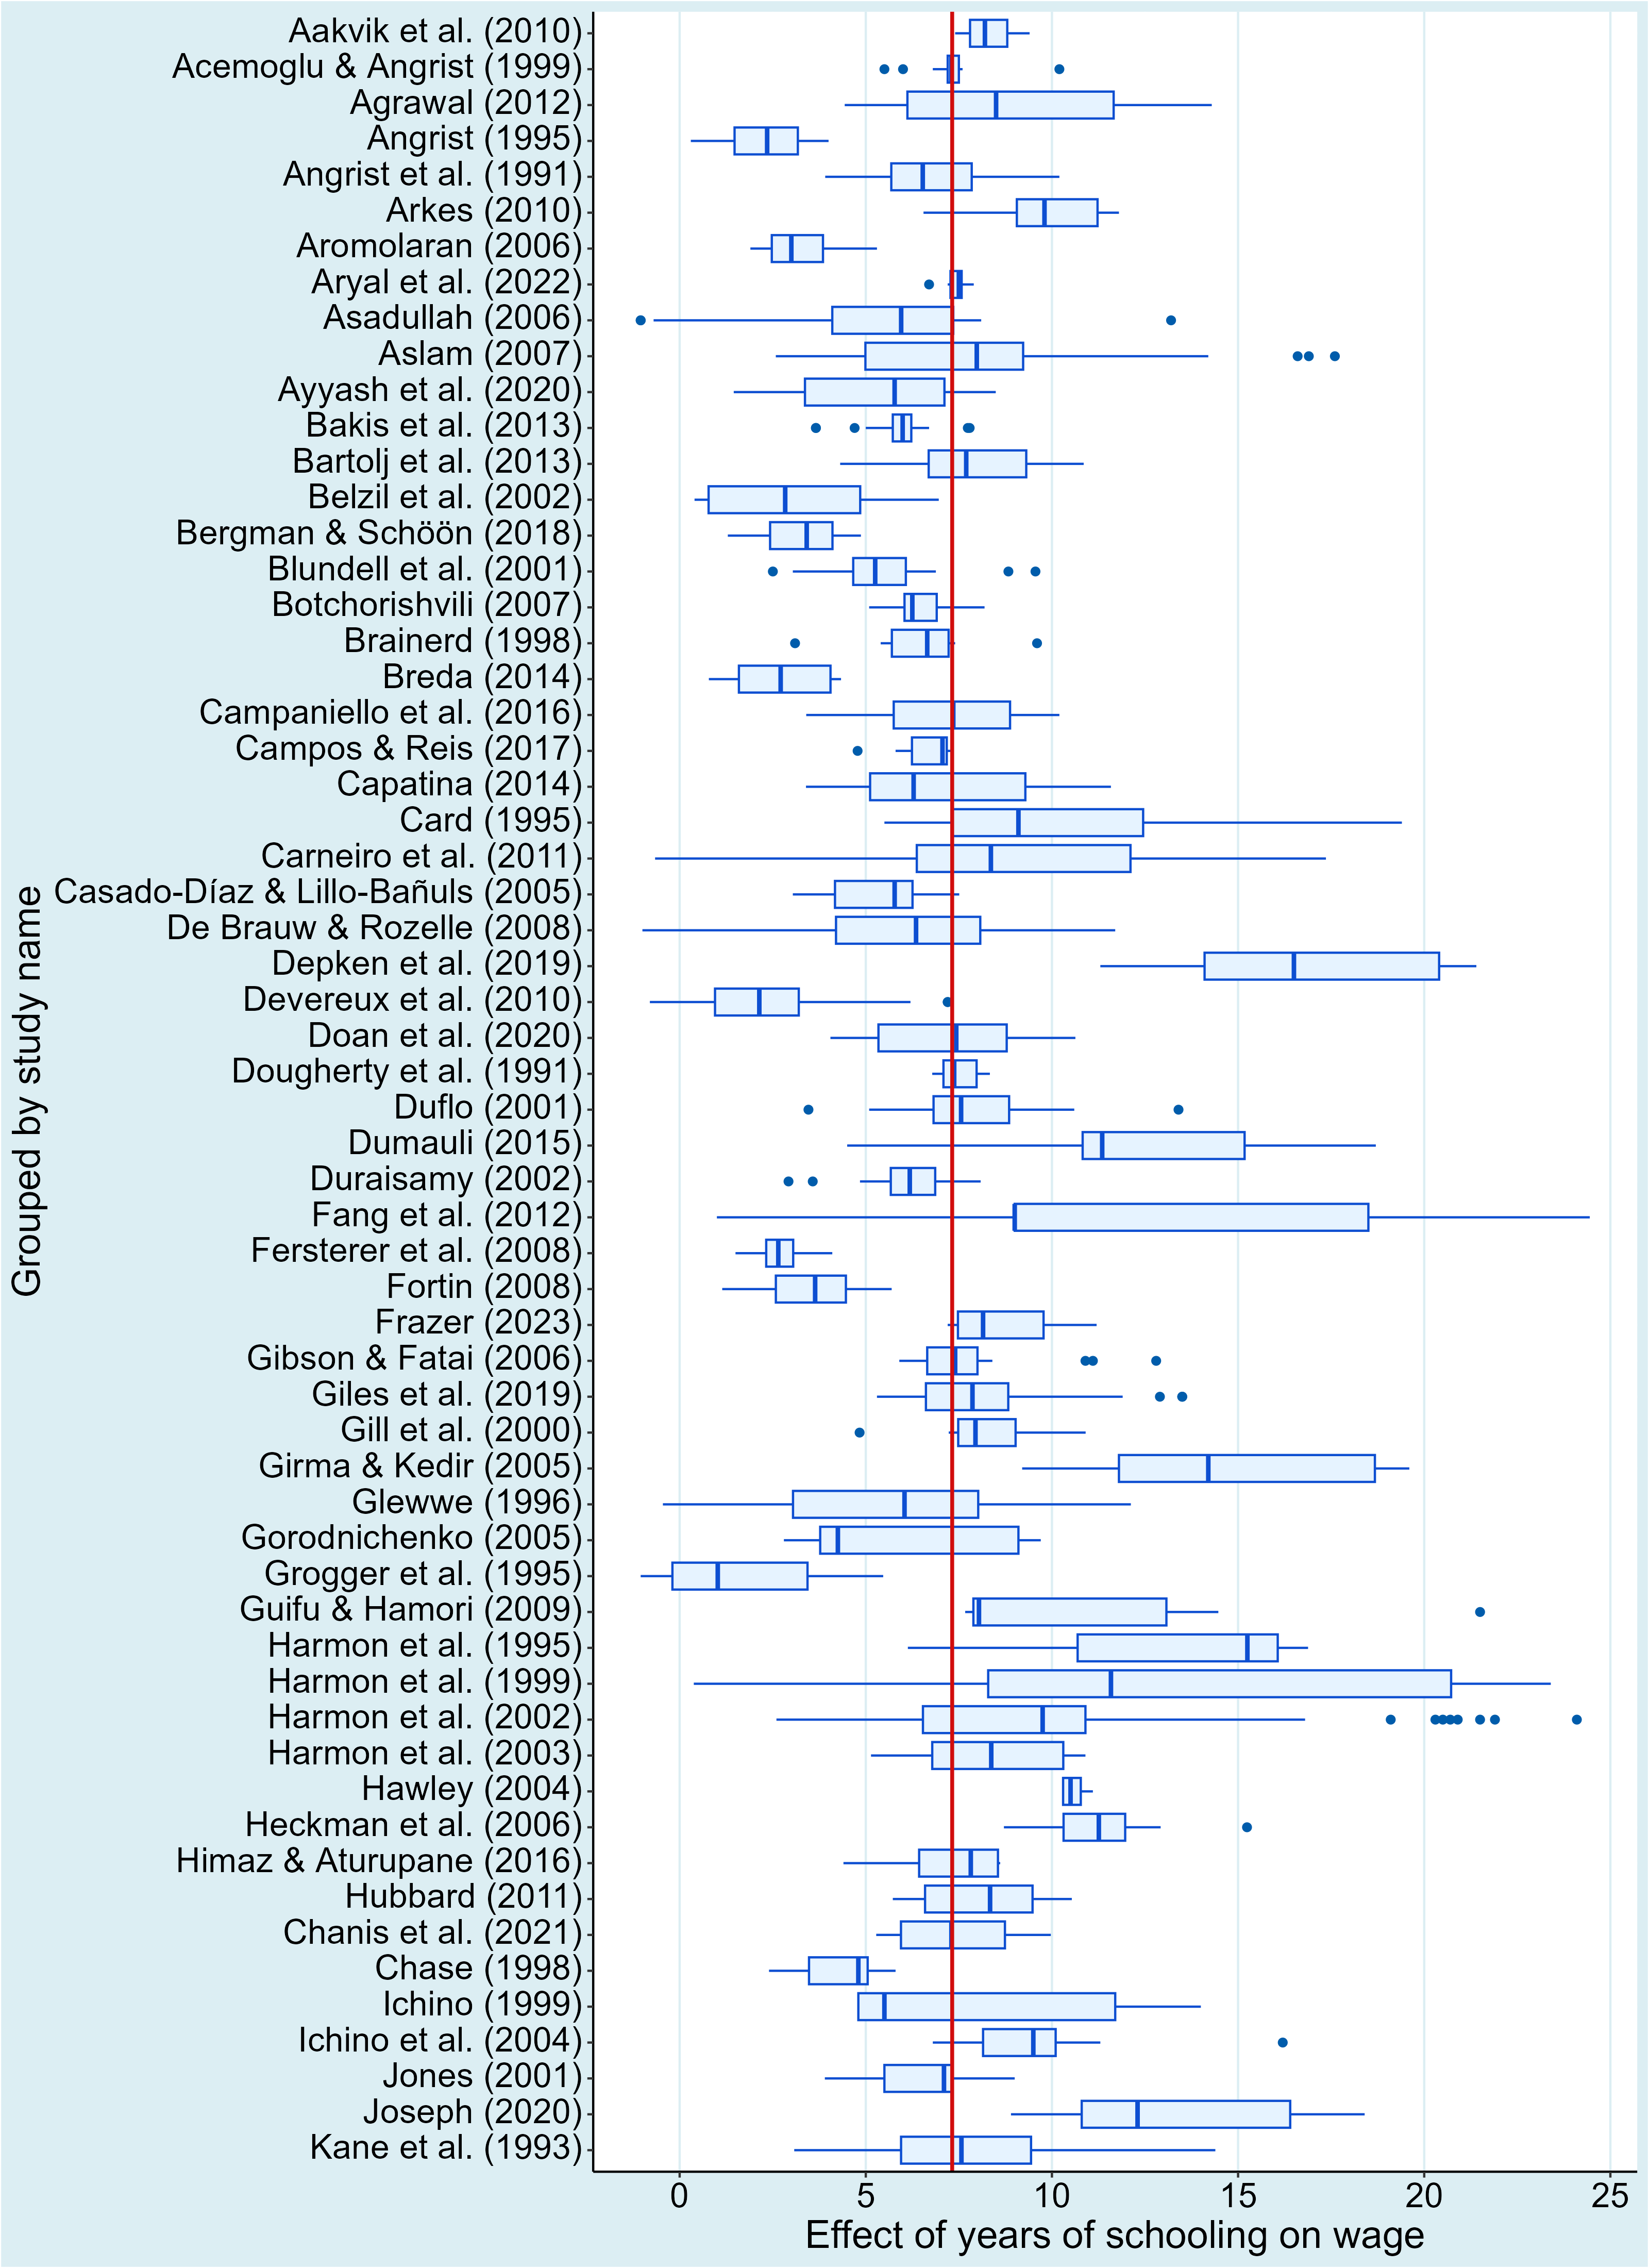
\includegraphics[width=0.9\textwidth]{Figures/box_plot_study_name_1.png}
      \end{center}\vspace{-0.7cm}
      \captionsetup{width=0.9\textwidth, font = scriptsize}
      \caption*{\emph{Note:} This figure shows the first part of a box plot, where the reported estimates are grouped at the study level. The first 60 studies from the dataset are displayed in alphabetically ascending order. The red line represents the average effect across the literature. Each box's length represents the interquartile range between the 25th and 75th percentiles. The dividing line within each box indicates the median value. The whiskers extend to the highest and lowest data points within 1.5 times the range between the upper and lower quartiles. Outliers are depicted as blue dots. The red line depicts the mean of the effect within the data. The data is winsorized at 1\% level.}
   \end{figure}
}
\afterpage{
   \begin{figure}[!t]
      \begin{center}
         \caption{Box plot of estimates across individual studies - second part}
         \label{fig:box_plot_studies_2}
         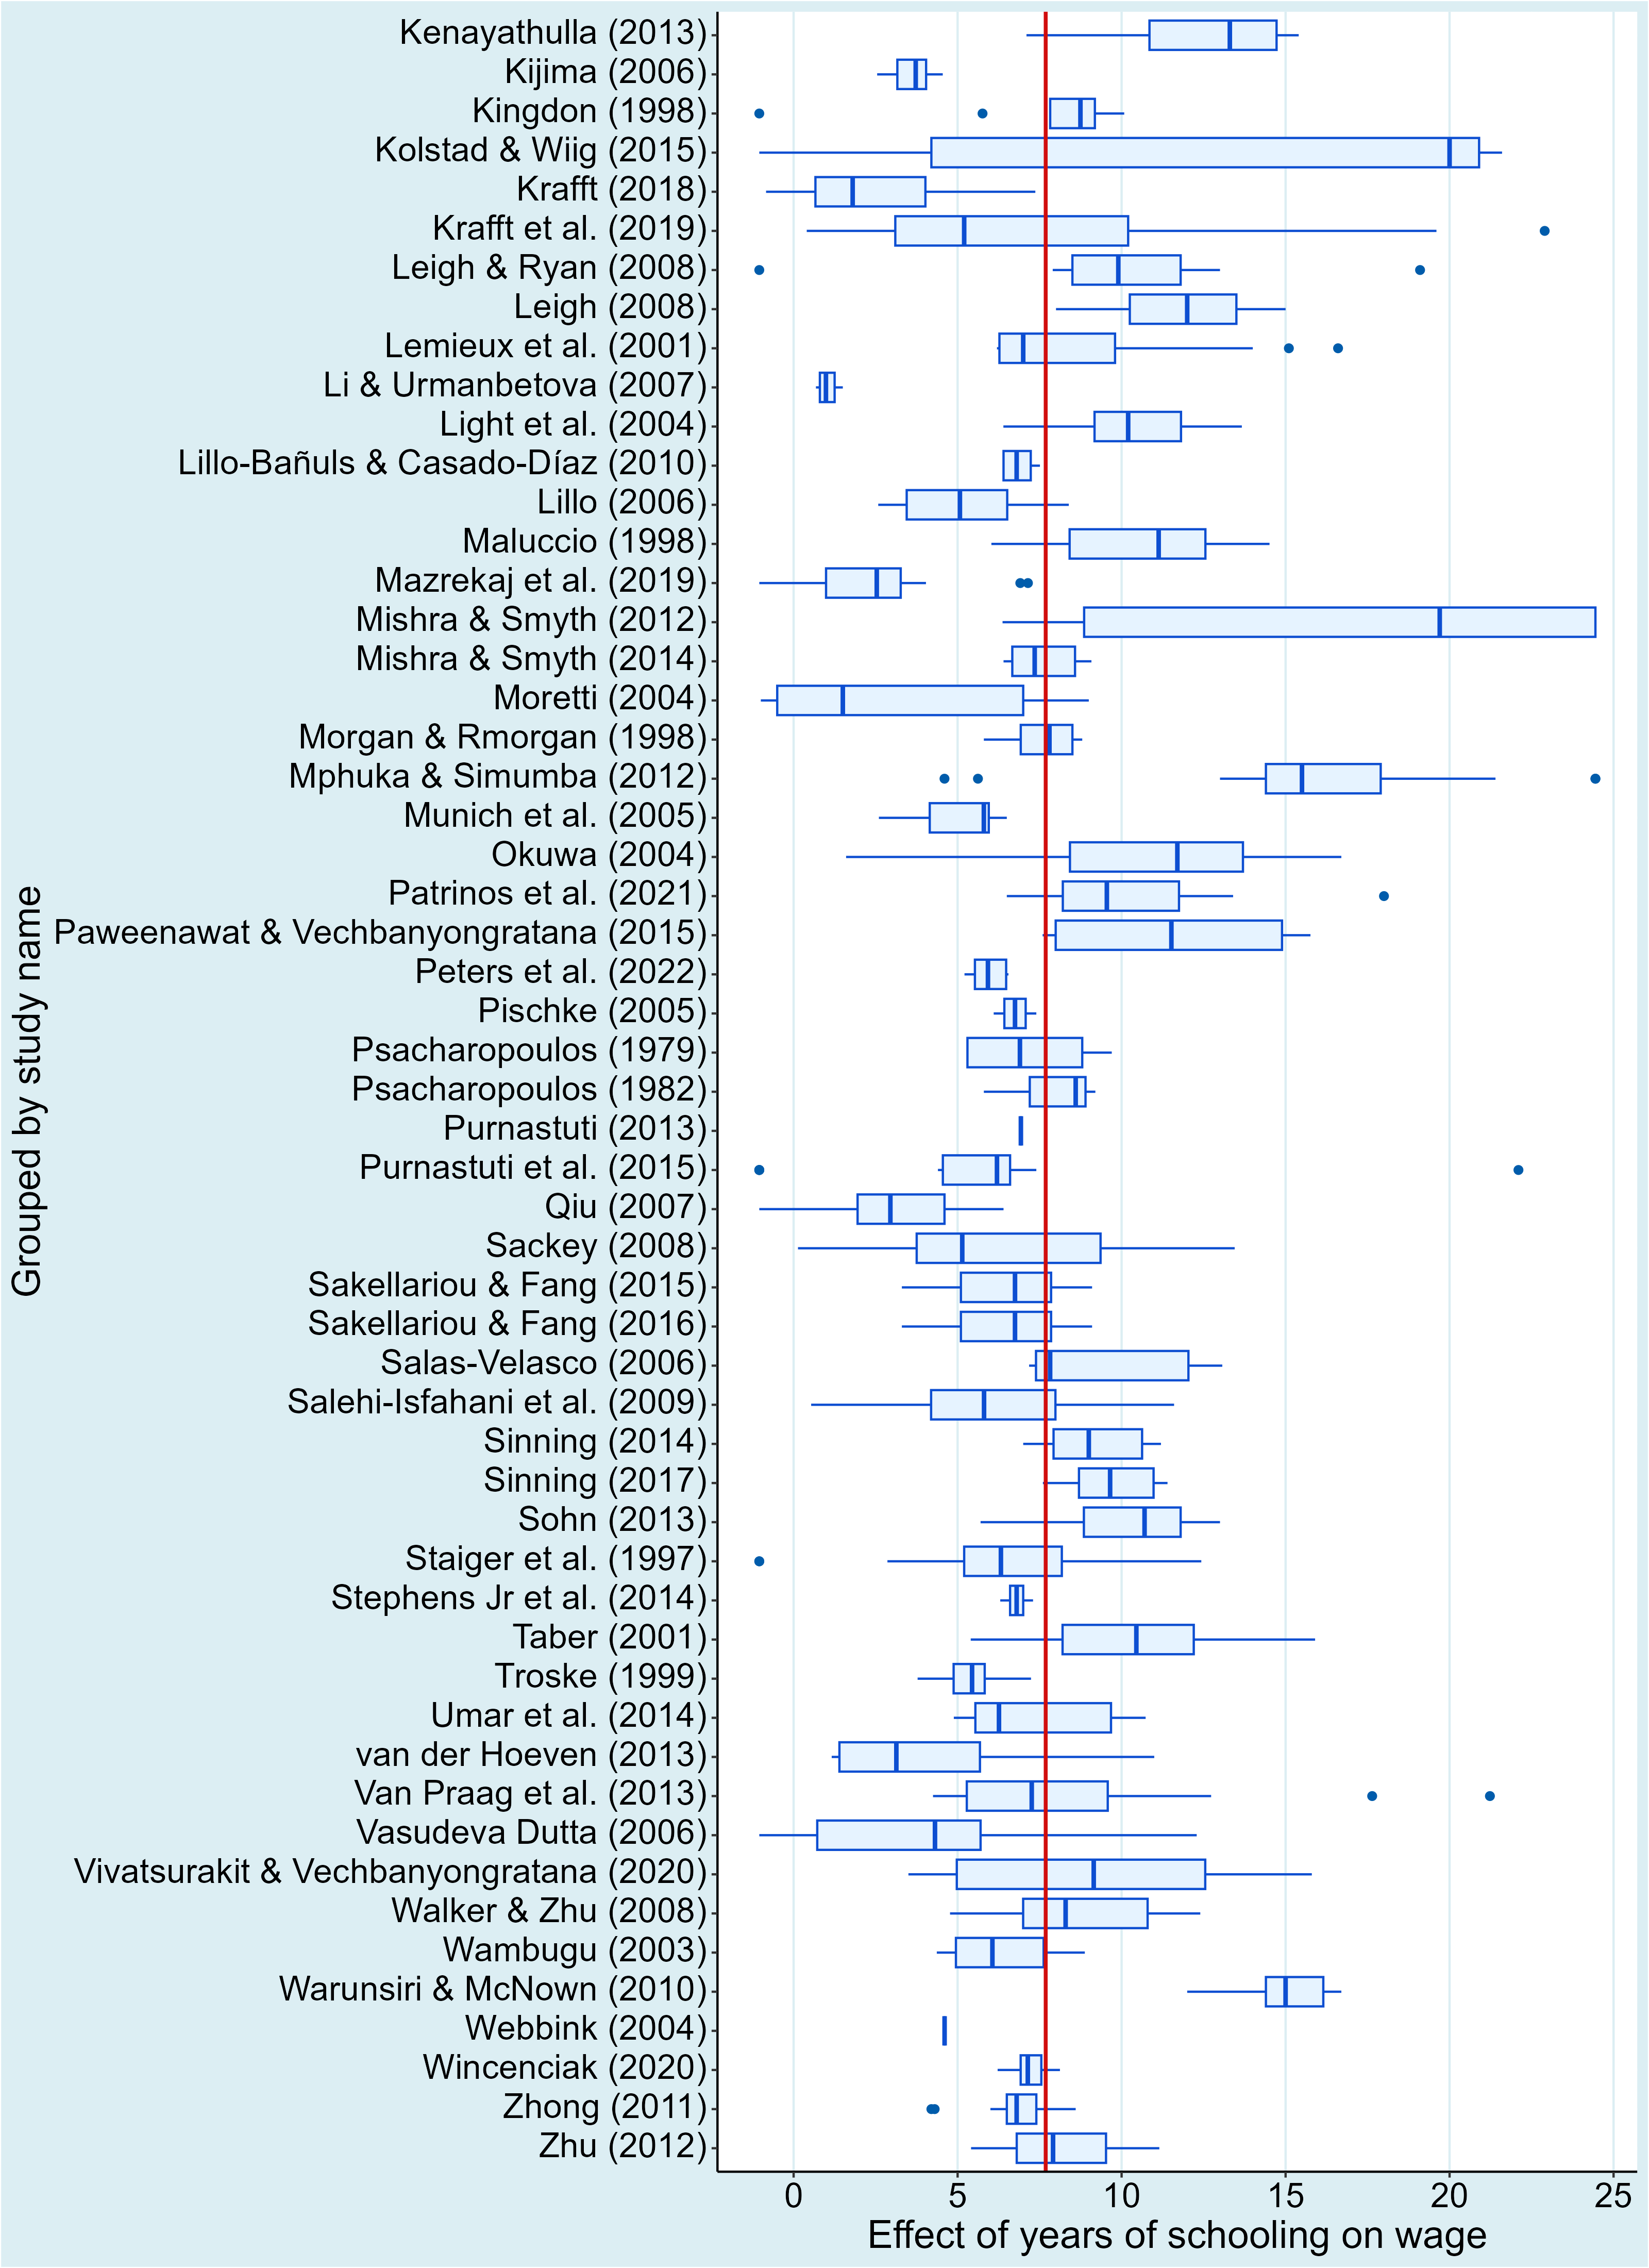
\includegraphics[width=0.9\textwidth]{Figures/box_plot_study_name_2.png}
      \end{center}\vspace{-0.7cm}
      \captionsetup{width=0.9\textwidth, font = scriptsize}
      \caption*{\emph{Note:} This figure shows the second part of a box plot, where the reported estimates are grouped at the study level. Fifty-five remaining studies from the dataset are displayed in alphabetically ascending order. The red line represents the average effect across the literature. Each box's length represents the interquartile range between the 25th and 75th percentiles. The dividing line within each box indicates the median value. The whiskers extend to the highest and lowest data points within 1.5 times the range between the upper and lower quartiles. Outliers are depicted as blue dots. The red line depicts the mean of the effect within the data. The data is winsorized at 1\% level.}
   \end{figure}
   \clearpage
}
